% =====================================================================
% A Joint Radio--Infrared--X-ray Bound on Bondi-fed Accretion onto the
% Candidate IMBH in Omega Centauri  (Paper F)
% Tim Swanson — The Omega Centauri Society / Post Oak Labs
% Build: pdflatex accretion-limit-paper && bibtex accretion-limit-paper
%        && pdflatex x2
% Posterior (computation of record): figs/fF_posterior_v4.py (seed 42)
%   -> figs/fF_v4_results.json, figs/fF_v4_exclfrac.json, figs/fF_v4_pgf.txt,
%      figs/fF_v4_scalings.json; seed study figs/fF_v4_addendum.py ->
%      figs/fF_v4_seedspread.json; standalone recomputes figs/fF_r9_checks.py
% v2.0 corrections per WU OCS-R9-F-1 (findings F-R9-01..07 and F-R8-01..16 of
%   OCS-PAPER-RIGOR-REVIEW_2026-09-03 / _2026-09-02): Xie & Yuan piecewise
%   efficiency with delta as an eighth nuisance, per-filter IR band-integration
%   correction, wind-supply recount (the n_e floor was a ceiling), and a
%   posterior-predictive reconstruction of P_excl.  v0.4 reproduces v0.3 to
%   floating-point equality with those corrections disabled; that is asserted
%   at run time.
% Superseded, retained in the chain: figs/fF_posterior_v3.py -> figs/fF_v3_results.json
%   and figs/fF_posterior_v2.py -> figs/fF_v2_results.json
% Measured-input provenance: figs/fF_measured_inputs.json (WU OCS-F-DATA-1)
% Appendix cross-check: figs/fF_joint_bound.py -> figs/fF_results.json
% v0.2 restructure per referee memos of 2026-08-13
% (OCS-REFEREE-F-REVIEW_2026-08-13.md): likelihood-based posterior,
% SED families, gas-supply floor, natural-expectation band, forecasts.
% v1.2 expansion per OCS-REFEREE-FGH-EXPANSION_2026-08-20.md items F-1..F-5
% (WU OCS-F-EXPAND-1): nuisance ladder, band adjudication figure, continuous
% exclusion curve, epoch-resolved duty-cycle analysis, DM requirement table.
% Expansion analyses: figs/fF_expand_v1.py -> figs/fF_expand_*.json,
%   figs/fF_expand_sed.png.  No v0.3 number is changed by that script; it
%   asserts the reproduced RIAF anchors against fF_v3_results.json at run time.
% v0.3 input corrections per figs/fF_v3_DELTA.md (WU OCS-F-V03-1):
% Haggard distance 5.2 kpc, X-ray limit at 95 per cent CL, per-filter
% Chen limits, epoch list, MAVERIC context.
% =====================================================================
\documentclass[11pt]{article}

\usepackage[margin=1.1in]{geometry}
\usepackage{newtxtext,newtxmath}
\usepackage[round,authoryear]{natbib}
\usepackage{graphicx}
\usepackage{booktabs}
\usepackage{amsmath}
\usepackage{tikz}
\usepackage{pgfplots}
\pgfplotsset{compat=1.17}
\usepgfplotslibrary{fillbetween}
\usepackage[font=small,labelfont=bf]{caption}
\usepackage{microtype}
\usepackage[colorlinks=true,linkcolor=blue!50!black,citecolor=blue!50!black,urlcolor=blue!50!black]{hyperref}
\usepackage{xcolor}

\newcommand{\msun}{\ensuremath{M_\odot}}
\newcommand{\ocen}{$\omega$~Cen}
\newcommand{\mdotB}{\ensuremath{\dot{M}_{\mathrm{B}}}}
\newcommand{\eps}{\ensuremath{\varepsilon_{\mathrm{B}}}}
\newcommand{\epsl}{\ensuremath{\varepsilon_{95}}}
\newcommand{\specbox}[1]{\par\smallskip\noindent\fbox{\parbox{0.97\linewidth}{\small\textbf{Epistemic status:} #1}}\smallskip\par}

\title{\textbf{A Joint Radio--Infrared--X-ray Bound on Bondi-fed Accretion onto the Candidate Intermediate-Mass Black Hole in Omega Centauri}}
\author{Tim Swanson\\[2pt]
\small The Omega Centauri Society / Post Oak Labs\\
\small \texttt{tim@postoaklabs.com}}
\date{August 2026 \\[4pt] \small v2.1 (last revised 2026-09-03) --- sixth paper of the set (Paper F); companion to the Macro Transcension\\ \small Hypothesis (Paper A), the inward-migration review (Paper B), the Omega Centauri campaign (Paper C),\\ \small the migration economics (Paper D), the engineered-IMBH systems paper (Paper E), the residual X-ray census (Paper G),\\ \small and the mass-tension paper (Paper H);\\ \small prepared for omegacentauri.me}

\begin{document}
\maketitle

\begin{abstract}
\noindent
Three deep non-detections now constrain any accretion flow onto the candidate intermediate-mass black hole (IMBH) at the center of Omega Centauri: a 170-hour ATCA radio campaign reaching 1.1\,$\mu$Jy rms at 7.25\,GHz \citep{Mahida2026}, JWST NIRCam/MIRI imaging showing no accretion-like point source at any proposed center \citep{Chen2025JWST}, and a 291-ks Chandra exposure bounding $L_X(0.5\text{--}7\,\mathrm{keV}) \leq 1.6\times10^{30}\,\mathrm{erg\,s^{-1}}$ \citep{Haggard2013}. \citet{Chen2025JWST} compare the infrared and radio limits qualitatively; no formal joint bound with propagated uncertainties has been published. We supply one, as a posterior. Defining the Bondi radiative efficiency $\eps \equiv L_{\mathrm{bol}}/(\mdotB c^{2})$, we build a forward model from $(\eps, M)$ and eight shared nuisance parameters (gas density, sound speed, distance, two SED band fractions, fundamental-plane scatter as a latent variable, inflow-suppression index, electron-heating fraction) to the three measured quantities, evaluate Gaussian likelihoods on the measurements themselves, and report the 95\,per~cent credible upper limit $\epsl(M)$ for three named accretion-flow families. For a radiatively inefficient (RIAF-like) flow, $\epsl = 2.9\times10^{-10}$ at the fast-star mass anchor of $8{,}200\,\msun$ and $1.1\times10^{-11}$ at $4\times10^{4}\,\msun$; removing the fundamental-plane radio leg entirely relaxes these to $1.4\times10^{-8}$ and $7.9\times10^{-10}$. Overplotting the expectation band for a natural outflow-suppressed hot flow at the same nuisance draws converts the curve into a calibrated verdict. Scoring each natural-flow draw against the measured data directly, the data reject 85\,per~cent of that parameter space at the fast-star anchor, 78\,per~cent at the pulsar-timing point-mass cap and 99\,per~cent at $4\times10^{4}\,\msun$ (28, 20 and 76\,per~cent using no radio information). A Bondi-fed hot flow at a 47~Tucanae-like density is therefore disfavoured across the contested mass range rather than only at its top, and something must give at every anchor: the mass, the gas density, or the suppression physics. Two of those figures replace weaker ones. Drafts of this paper to v1.5 reported 31 and 90\,per~cent at the two upper anchors and a natural flow surviving comfortably at the fast-star anchor; that reading rested on an efficiency law linear in accretion rate where the fits it cited are close to square-root, and on an exclusion statistic that compared the natural draws against a limit marginalized over those same draws. Both are corrected here and both move the verdict the same way. The strengthened claim is also the more fragile one, since the corrected efficiency law is extrapolated three to five decades below the rates it was computed for; holding it flat at the edge of its computed range instead drives every figure above 99\,per~cent, so the extrapolation is the conservative end of the bracket rather than the optimistic one. The limit's normalization is conditional on the unmeasured central gas density throughout, and we quantify that dependence three ways: prior-widening and prior-shift tests (factor $\sim$6 each), a stellar-wind budget that bounds the density from above rather than below once its giant census is recounted, and a forecast showing that a pulsar dispersion-measure determination of the core density, feasible with the current 19-pulsar timing set, would harden the entire curve. The single observation that converts these limits from analogy-conditional to measured is a DM-gradient fit to the 19-pulsar set at the $\pm10$ per cent level (\S8.1). Resolving the radio campaign into the 25 observing blocks its source paper tabulates also converts the duty-cycle loophole from an acknowledgement into a bounded region: a train of $100\,\mu$Jy flares lasting 2\,hr is excluded for recurrence intervals shorter than 31\,hr, while a 1\,mJy flare lasting half an hour escapes the whole campaign if it recurs less often than every 3.4\,days, a duty cycle of $6\times10^{-3}$. All results derive from a fixed-seed Monte Carlo shipped with the paper.
\end{abstract}

\bigskip
\noindent\textbf{Keywords:} intermediate-mass black holes; Omega Centauri; NGC 5139; Bondi accretion; radiatively inefficient accretion flows; fundamental plane of black hole activity

\newpage
\tableofcontents
\newpage

\section{Introduction}
\label{sec:intro}

Omega Centauri hosts the nearest strong IMBH candidate: fast-moving stars inside the central arcsecond require an enclosed dark mass $\gtrsim 8{,}200\,\msun$ \citep{Haberle2024Nature}, while pulsar-timing and kinematic modeling favor an extended dark remnant component of $\sim 2\text{--}3\times10^{5}\,\msun$ and cap any point mass at $\lesssim 6{,}000\,\msun$ at $3\sigma$ \citep{BanaresHernandez2025}, a tension sharpened rather than resolved by the current 19-pulsar timing set \citep{ColomiBernadich2026}. The center is electromagnetically silent at the depths quantified below. The radio silence has a two-decade history: upper limits of $\sim 100\,\mu$Jy at GHz frequencies \citep{Maccarone2005}, a $2.5\sigma$ near-center excursion flagged as worth deeper follow-up \citep{LuKong2011}, JVLA limits of 1.5--2.1\,$\mu$Jy\,beam$^{-1}$ in three other clusters that set the methodological template for radio IMBH searches \citep{Strader2012}, the 50-cluster MAVERIC survey null \citep{Tremou2018}, and now the deepest radio image of any globular cluster, 170 hours with ATCA reaching 1.1\,$\mu$Jy rms at 7.25\,GHz with no source at any proposed center and the nearest $5\sigma$ source 13 arcseconds away \citep{Mahida2026}. The \citet{LuKong2011} excursion does not recur at a factor $\sim$6 deeper in rms; the $2.5\sigma$ peak they flagged would have registered at $\gtrsim14\sigma$ in the new image, which retires that thread. In the infrared, JWST NIRCam and MIRI imaging of the core shows no point source with an accretion-like spectral energy distribution \citep{Chen2025JWST}; in X-rays, the combined 291-ks Chandra exposure gives $L_X \leq 1.6\times10^{30}\,\mathrm{erg\,s^{-1}}$, which \citet{Haggard2013} translated to accretion efficiencies spanning $10^{-5}$--$10^{-9}$ across the $3\times10^{3}$--$3\times10^{4}\,\msun$ mass window they consider. Their abstract also rounds that span to $10^{-6}$--$10^{-8}$; drafts of this paper to v1.5 quoted the rounded form as though it were the source's range, and the wider figure is the one their text states.

\citet{Chen2025JWST} place their infrared limits alongside the radio limits and note that the radio is the more restrictive at the high-mass end (their Figure~7). That comparison is qualitative: each band's limit is quoted under its own model assumptions, at its own fiducial mass, with no shared error budget. The three limits constrain three different quantities, a radio flux routed through a jet or fundamental-plane relation, a band-limited infrared luminosity, and a band-limited X-ray luminosity, and all three depend on the same unmeasured gas density, the same contested black-hole mass, and the same distance. Multiplying or stacking them as if independent would overstate the joint constraint; quoting any of them at a single mass begs the question the mass tension leaves open.

This paper supplies the missing joint analysis, and in doing so surfaces a result the single-band treatments could not state: the combined data are now deep enough to exclude most of the parameter space of a natural Bondi-fed hot flow across the contested mass range. Section~\ref{sec:data} fixes the observational inputs; Section~\ref{sec:method} the forward model, the likelihoods, and the three accretion-flow families; Section~\ref{sec:gas} the gas-supply physics that bounds the dominant nuisance from above; Section~\ref{sec:results} the posterior curves, the natural-flow comparison, and the prior-sensitivity budget; Section~\ref{sec:duty} the duty-cycle loophole; Section~\ref{sec:forecast} forecasts; and Section~\ref{sec:discussion} what the bound adjudicates. Appendix~\ref{app:conventions} collects every unit conversion and convention; Appendix~\ref{app:mincheck} retains the simpler threshold-inversion construction of an earlier draft as a transparent cross-check. The Monte Carlo script, its fixed seed, and its full output accompany the paper.

\section{Observational inputs}
\label{sec:data}

\textbf{Radio.} \citet{Mahida2026}: ATCA project CX556 plus archival data, $\sim$170\,h at 5.5 and 9.0\,GHz combining to an effective 7.25\,GHz image with rms $\sigma_S = 1.1\,\mu$Jy\,beam$^{-1}$; no detection at any of their three tested centers, A, B, and C, coincident with though not labelled as the \citet{vanderMarelAnderson2010} and \citet{Noyola2008,Noyola2010} centers. We treat the central flux density as measured to be $0 \pm \sigma_S$.

\textbf{Infrared.} \citet{Chen2025JWST}: JWST NIRCam and MIRI imaging of the core with no accretion-like point source. Their Table~1 states a limiting luminosity per filter at each of three completeness levels, and we use those numbers directly rather than a single band-summary constant (Table~\ref{tab:irfilters}). Each filter enters the likelihood as its own Gaussian term on the predicted band-peak $\nu L_{\nu}$, at the 95\,per~cent completeness row, the row that matches the X-ray leg's stated confidence. Their tabulated limits are band-integrated, as their own definition $L = 4\pi d^{2}F_{\lambda}\Delta\lambda$ states, so each $\sigma_{j}$ carries the conversion between the two quantities as well as the quantile: $\sigma_{j} = (\lambda_{c}/\Delta\lambda)\,L_{\mathrm{lim},j}/1.645$, a factor of 4.0 to 5.6 per filter (Table~\ref{tab:irfilters}). Drafts to v1.5 compared the band-peak prediction against the band-integrated limit directly, which made the infrared terms tighter than the data support by that factor; correcting it loosens the RIAF anchors by 4 to 7\,per~cent, the jet anchors by 32 to 37\,per~cent and the radio-free anchors by 60\,per~cent. Completeness is a detection-recovery fraction rather than a confidence level, so reading it through the normal quantile is a convention; the 99.7 and 68\,per~cent rows are run alongside and are reported in Appendix~\ref{app:conventions}. F770W dominates the combination. Treating four filters as independent terms is optimistic, since they observe one source: the conservative reading, which keeps only the tightest single filter, sits within 2\,per~cent of the combination on the jet family and 6\,per~cent on the RIAF family, so nothing here rests on the independence assumption. A second correction to the same table is disclosed rather than made silently. The 99.7\,per~cent completeness row for F200W is transcribed in the provenance file with a luminosity entry equal to its flux entry, which breaks the ratio $L/F_{\lambda}$ that the filter's other three rows share to 1\,per~cent; the value that ratio implies, $7.5\times10^{31}\,\mathrm{erg\,s^{-1}}$, is used in the 99.7\,per~cent ladder row of Appendix~\ref{app:conventions}. That row is not the primary one and no headline number depends on it. Limits are referenced at \citeauthor{Chen2025JWST}'s adopted 5.49\,kpc and rescaled to the drawn distance. \citet{Chen2025JWST} state their accretion constraint for $M \lesssim 10^{4}\,\msun$, so the $4\times10^{4}\,\msun$ anchor extrapolates their stated range by a factor of four; the SED-family treatment of Section~\ref{sec:families} is what carries that anchor, and the radio-free curve there should be read with this caveat attached.

\begin{table}[tbp]
\centering
\small
\caption{JWST per-filter limits adopted for the infrared leg, from \citet{Chen2025JWST}, their Table~1, at the 95\,per~cent completeness row, at their adopted distance of 5.49\,kpc. $L_{\mathrm{lim}}$ is band-integrated, as that table's own definition $L = 4\pi d^{2} F_{\lambda}\Delta\lambda$ states. $\Delta\lambda$ is not printed in the source and is recovered from the ratio $L/F_{\lambda}$ across that filter's completeness rows, which agree to 1--6\,per~cent. The likelihood predicts a band-peak $\nu L_{\nu}$, so the conversion between the two enters each filter's term: $\sigma_{j} = (\lambda_{c}/\Delta\lambda)\,L_{\mathrm{lim},j}/1.645$ (\S\ref{sec:likelihood}). Drafts to v1.5 omitted that factor and compared a band-peak prediction against a band-integrated limit.}
\label{tab:irfilters}
\begin{tabular}{lccccc}
\toprule
Filter & Vega mag limit & $L_{\mathrm{lim}}$ ($\mathrm{erg\,s^{-1}}$) & $\Delta\lambda$ (\AA) & $\lambda_{c}/\Delta\lambda$ & $\sigma_{j}$ ($\mathrm{erg\,s^{-1}}$) \\
\midrule
F200W  & $>20.8$ & $4.8\times10^{30}$ & $4{,}720$ & 4.24 & $1.24\times10^{31}$ \\
F444W  & $>17.8$ & $9.2\times10^{30}$ & $11{,}090$ & 4.00 & $2.24\times10^{31}$ \\
F770W  & $>17.5$ & $1.9\times10^{30}$ & $14{,}985$ & 5.14 & $5.94\times10^{30}$ \\
F1500W & $>14.5$ & $4.9\times10^{30}$ & $26{,}850$ & 5.59 & $1.66\times10^{31}$ \\
\bottomrule
\end{tabular}
\end{table}

\begin{sloppypar}
\textbf{X-ray.} \citet{Haggard2013}: 290.9\,ks of Chandra ACIS data, $f_X(0.5\text{--}7\,\mathrm{keV}) \leq 5.0\times10^{-16}\,\mathrm{erg\,cm^{-2}\,s^{-1}}$ absorption-corrected. \citet{Haggard2013} quote this at 95\,per~cent confidence and never write a $\sigma$; their \texttt{aprates} bound is on a non-negative count rate, so we read it as one-sided and take the measured central flux as $0 \pm f_{X,\mathrm{lim}}/1.645$. An earlier draft of this paper labelled the limit $3\sigma$ and used $f_{X,\mathrm{lim}}/3$, which is not the source's convention. The two-sided 95\,per~cent and the $f_{X,\mathrm{lim}}/3$ readings are carried as a ladder in Appendix~\ref{app:conventions}; they span 5\,per~cent on the RIAF anchors, so the choice inside the ladder is not load-bearing.
\end{sloppypar}

\textbf{Positional coverage.} The proposed centers \citep{vanderMarelAnderson2010,Noyola2008,Noyola2010} differ by over an arcsecond, and the hole wanders about the potential minimum with r.m.s. amplitude $\lesssim 10^{-2}$\,pc, about $0.4''$ at 5.43\,kpc, with a leptokurtic distribution whose excursions reach $1$--$2''$ more often than a Gaussian would allow \citep{DiCintio2023,ChatterjeeHernquistLoeb2002}. None of this strains the limits; the reason is independent of beaming: each dataset images or covers the entire core region at its quoted depth, and in the radio the nearest $5\sigma$ source of any kind lies $13''$ from Center B, in \citeauthor{Mahida2026}'s own phrasing \citep{Mahida2026}. Every position in the center list, and the full wander tail, inherits the per-band limits; no positional correction enters the error budget. The distance used here, $5.43\,\mathrm{kpc}$, is this paper's own likelihood input (Table~\ref{tab:priors}); the companion papers in the set adopt $5.49\,\mathrm{kpc}$ as the set fiducial, and the resulting offset, 1.2\,$\sigma$ of this paper's distance prior, is disclosed in \S\ref{sec:priors} rather than harmonized away.

\section{Method}
\label{sec:method}

\subsection{Definitions and conventions}
\label{sec:defs}

Let $\mdotB$ be the Bondi capture rate from gas at rest in the cluster core,
\begin{equation}
\mdotB = 4\pi \lambda\,\frac{(GM)^{2}\rho_{\mathrm{gas}}}{c_{s}^{3}},
\qquad \lambda(\gamma{=}5/3) = 0.25 \citep{Bondi1952},
\label{eq:bondi}
\end{equation}
with $\rho_{\mathrm{gas}} = \mu_{e} m_{p} n_{e}$ and $\mu_{e} = 1.17$ for an ionized plasma of solar-like composition. Gas in hydrostatic equilibrium shares the cluster's rest frame, and the hole's Brownian velocity, $\sigma(m_{*}/M)^{1/2} \sim 0.1\,\mathrm{km\,s^{-1}}$, is negligible against $c_{s}$, so no bulk-velocity term enters the denominator; this is the convention of the comparison literature \citep{Strader2012,Tremou2018,Haggard2013}. A variant that treats the stellar velocity dispersion as a turbulent-velocity proxy in the denominator, the convention of Paper E's fuel budget, is evaluated in Appendix~\ref{app:conventions}; it lowers $\mdotB$ by a factor $\simeq 1.9$ net of the eigenvalue and weakens every limit by the same factor.

We define the \emph{Bondi radiative efficiency}
\begin{equation}
\eps \equiv \frac{L_{\mathrm{bol}}}{\mdotB c^{2}},
\end{equation}
the bolometric radiative output per unit of captured rest-mass energy, the quantity the data constrain directly. It factors as $\eps = \eta\, f_{\mathrm{B}}$, with $f_{\mathrm{B}}$ the fraction of captured gas reaching the horizon and $\eta$ the radiative efficiency of the arriving flow. In natural hot flows the inflow declines inward, $\dot{M}(R) \propto R^{s}$, with $0 \le s \le 1$ admissible on general grounds \citep{BlandfordBegelman1999} and modeled values spanning $s \simeq 0.3$--$0.8$ \citep{YuanNarayan2014}; we adopt $s \in [0.3, 0.5]$ as this paper's working sub-range within that modeled span. With $r_{\mathrm{B}} = GM/c_{s}^{2}$ and the gravitational radius $r_{g} = GM/c^{2}$, so that $r_{\mathrm{B}}/r_{g} = (c/c_{s})^{2}$ and the bracket depends on $c_{s}$ and $s$ alone,
\begin{equation}
f_{\mathrm{B}} = \left(\frac{r_{\mathrm{B}}}{r_{g}}\right)^{-s} \in [10^{-4.4},\,10^{-2.6}]
\quad\text{for } s \in [0.3, 0.5],
\end{equation}
consistent with Paper E's fiducial $s \simeq 0.3$ suppression of $\sim 500$ at $2\times10^{4}\,\msun$. Published per-band efficiencies use other conventions: \citet{Mahida2026} bound a model-specific accretion fraction ($\lesssim 4\times10^{-3}$), \citet{Haggard2013} an efficiency under fixed gas density and mass ($10^{-5}$--$10^{-9}$ over their stated mass window). Appendix~\ref{app:conventions} prints the conversion table; none of those numbers is $\eps$, and no direct numerical comparison should be made without it.

\subsection{Shared nuisance parameters}
\label{sec:priors}

Table~\ref{tab:priors} lists the priors. One draw of the full vector serves all three bands in each realization: the gas density that scales the radio prediction is the same density that scales the infrared and X-ray ones, the SED fraction $f_{X}$ that converts the X-ray measurement also drives the fundamental-plane prediction (the two legs constrain the same source's SED, so drawing $f_{X}$ once induces the correlation reality does), and the distance rescales all three measured quantities together.

\begin{table}[tbp]
\centering
\small
\caption{Monte Carlo priors ($4\times10^{4}$ draws, fixed seed; script \texttt{figs/fF\_posterior\_v4.py}). SED band fractions are family-specific (Table~\ref{tab:families}).}
\label{tab:priors}
\begin{tabular}{llp{5.6cm}}
\toprule
Parameter & Prior & Basis \\
\midrule
$n_{e}$ & log-normal, median $0.23\,\mathrm{cm^{-3}}$, 0.5\,dex & 47 Tuc analogy \citep{Freire2001,Abbate2018}; \S\ref{sec:gas} \\
$c_{s}$ & uniform, 11.7--16.6\,$\mathrm{km\,s^{-1}}$ & $10^{4}$\,K photoionized gas, isothermal ($\mu{=}0.6$) to adiabatic (pure H) \\
$d$ & normal, $5.43 \pm 0.05$\,kpc & cluster distance; rescales all bands \\
$f_{X}, f_{\mathrm{IR}}$ & family-specific (Table~\ref{tab:families}) & hot-flow SED literature \\
FP latent offset & normal, 0 $\pm$ 0.88\,dex & fundamental-plane intrinsic scatter \citep{Merloni2003} \\
$s$ & uniform, 0.3--0.5 & inflow-suppression index \citep{YuanNarayan2014}; Paper E fiducial 0.3; enters $\varepsilon_{\mathrm{nat}}$ only, not the likelihood (\S\ref{sec:nuisance}) \\
$\delta$ & uniform over $\{10^{-3}, 10^{-2}, 0.1, 0.5\}$ & electron-heating fraction; the four values \citet{XieYuan2012} tabulate, drawn discretely because the efficiency fit exists only at those values; enters $\varepsilon_{\mathrm{nat}}$ only (\S\ref{sec:eta}) \\
$\sigma$ & fixed, 21\,$\mathrm{km\,s^{-1}}$ & paper-set fiducial (enters $r_{\mathrm{infl}}$ only) \\
\bottomrule
\end{tabular}
\end{table}

The gas density is the weakest input and it multiplies everything, so its treatment is spread across three places: the prior here (a 47 Tucanae analogy, since \ocen{} has no direct ionized-gas measurement; the one \ocen-specific figure, $n_{e} = 1.94\,\mathrm{cm^{-3}}$ from sodium absorption, is flagged by its authors as a foreground-dominated upper limit and is not used; \citealt{oMEGACatVII2025}), the wind budget of Section~\ref{sec:gas}, which bounds the local supply from above, and the sensitivity budget of Section~\ref{sec:sensitivity}. \citet{Mahida2026} adopt $n_{e} = 0.2 \pm 0.1\,\mathrm{cm^{-3}}$ for the same cluster on the same kind of reasoning, from pulsar-derived electron densities in other globular clusters, which is an independent arrival at the median used here and an indication of how narrow the defensible range is once the analogy is accepted at all. Every predicted flux in the forward model scales linearly with $n_{e}\eps$, so the data constrain the product, and the normalization of every curve in this paper is conditional on the $n_{e}$ prior. Every part of the $\eps$ curve depends on the 47 Tuc analogy; what can be done, and is done below, is to bound the analogy's plausible range astrophysically and to show the answer across that range.

One further input is disclosed rather than changed. The distance prior is the paper set's fiducial $5.43 \pm 0.05$\,kpc, while \citet{Mahida2026} adopt the kinematic distance $5.494 \pm 0.061$\,kpc. The offset is 1.2\,$\sigma$ of the prior and would loosen every leg by about 2\,per~cent, since a more distant source is fainter at fixed luminosity and every predicted flux falls. We hold the fiducial value across this paper set rather than harmonize it silently per paper, and record the direction and size of the effect here so that a reader who prefers the larger distance can apply it.

\subsection{Forward model and likelihoods}
\label{sec:likelihood}

For each trial $(\eps, M)$ and nuisance draw $\theta$: $L_{\mathrm{bol}} = \eps\,\mdotB(M,\theta)\,c^{2}$. The predicted observables are
\begin{align}
f_{X}^{\mathrm{pred}} &= f_{X} L_{\mathrm{bol}} / (4\pi d^{2}), \\
(\nu L_{\nu})^{\mathrm{pred}}_{\mathrm{IR}} &= f_{\mathrm{IR}} L_{\mathrm{bol}}, \\
\log L_{R}^{\mathrm{pred}} &= 0.60\,\log\!\big(k\,f_{X} L_{\mathrm{bol}}\big) + 0.78\,\log (M/\msun) + 7.33 + \delta_{\mathrm{FP}},
\end{align}
where $k = 0.610$ converts the 0.5--7\,keV band fraction to the 2--10\,keV band the fundamental plane is calibrated in (power law, $\Gamma = 2$; \citeauthor{Haggard2013}'s own $\Gamma = 2.3$ gives $k = 0.462$ and is carried as a ladder row in Appendix~\ref{app:conventions}), and $\delta_{\mathrm{FP}} \sim \mathcal{N}(0, 0.88\,\mathrm{dex})$ is the plane's intrinsic scatter as a latent variable. The plane is used only in the forward direction, the direction it was fit in \citep{Merloni2003}; no inverse regression is performed, which removes the calibration-problem objection that attaches to algebraic inversion of a scattered forward relation \citep{Plotkin2012}. The likelihood is the product of six Gaussians on the measured values: central radio flux density $0 \pm 1.1\,\mu$Jy, central X-ray flux $0 \pm f_{X,\mathrm{lim}}/1.645$, and four infrared band-peak luminosities $0 \pm \sigma_{j}$ from Table~\ref{tab:irfilters}, the infrared terms rescaled to the drawn distance from \citeauthor{Chen2025JWST}'s 5.49\,kpc. Where a band's published product is a limit rather than a measured value, a Gaussian whose $\sigma$ is that limit divided by the quantile of the confidence the source itself states is the reconstruction we adopt for the two legs published as limits, and Appendix~\ref{app:conventions} measures what it costs; the data-availability section requests exactly those numbers from the source teams, and the machinery ingests them unchanged.

The posterior at each $M$ is computed as the plain Monte Carlo mean of the likelihood over the $4\times10^{4}$ nuisance draws, which is an unweighted average because the draws come from the prior itself and no proposal reweighting is applied, on a log-spaced $\eps$ grid ($10^{-14}$--$10^{-2}$, log-uniform prior), and \epsl{} denotes the 95\,per~cent credible upper limit of the normalized posterior. Re-running the anchors under eight nuisance seeds, each with its own $\delta$ stream, puts the Monte Carlo spread of \epsl{} at 1.4 to 9.6\,per~cent of the mean across the three anchors and the three families, widest for the RIAF family and narrowest for the radio-free curve, and the spread of $P_{\mathrm{excl}}$ at 0.13 to 0.88 percentage points. Both sit an order of magnitude under the analysis-choice ranges of Section~\ref{sec:sensitivity}. The seed of record sits at the low end of the \epsl{} range and the high end of the $P_{\mathrm{excl}}$ range; the eight-seed minima and maxima ship in \texttt{figs/fF\_v4\_seedspread.json}. Upper limits from non-detections are sensitive to the prior's lower cutoff; Section~\ref{sec:sensitivity} quantifies that dependence (a factor of 9 to 40 when the floor rises from $10^{-14}$ to $10^{-11}$) and every quoted \epsl{} states its grid. This likelihood product, not a distribution of inverted thresholds, is what Paper E's Bayesian adjudication machinery consumes; the marginal likelihood over $\eps$ ships as a machine-readable table with the source.

\subsection{Accretion-flow families}
\label{sec:families}

A single SED bracket cannot serve all flows, and under a common bracket for $f_{X}$ and $f_{\mathrm{IR}}$ the X-ray leg dominates the infrared leg in every draw, leaving JWST unconstraining in this band; an earlier draft of this paper had exactly that structure, and the referee who caught it was right that it made the three-band claim cosmetic. We therefore evaluate three named families with distinct band-fraction priors (Table~\ref{tab:families}): a radiatively inefficient ADAF-like flow (X-ray-bright among the bands considered), a jet-dominated, synchrotron-peaked flow (infrared-bright, X-ray-faint, the family in which the infrared leg comes closest to binding), and a thin disk (radiatively efficient; included so the reader sees by how many decades it is excluded, and evaluated without the fundamental-plane leg since the plane is a hard-state/quiescent relation).

\begin{table}[tbp]
\centering
\small
\caption{Accretion-flow families. Band fractions are log-uniform within the stated ranges, set conservatively by construction to bracket each family's characteristic SED shape rather than fit to a specific source.}
\label{tab:families}
\begin{tabular}{lccc}
\toprule
Family & $f_{X}$ (0.5--7 keV) & $f_{\mathrm{IR}}$ (band peak) & radio leg \\
\midrule
RIAF (ADAF-like) & 0.03--0.3 & 0.03--0.3 & fundamental plane \\
Jet-dominated & 0.01--0.1 & 0.1--0.5 & fundamental plane \\
Thin disk & 0.05--0.2 & 0.05--0.3 & none \\
\bottomrule
\end{tabular}
\end{table}

\subsection{The natural-flow expectation and its efficiency law}
\label{sec:eta}

The limit curve becomes a verdict only against a prediction, and the prediction is $\varepsilon_{\mathrm{nat}} = \eta_{\mathrm{ADAF}}(\dot{m}_{\mathrm{hor}})\,f_{\mathrm{B}}$, with $\dot{m}_{\mathrm{hor}} = f_{\mathrm{B}}\mdotB/\dot{M}_{\mathrm{Edd}}$ the rate reaching the horizon in Eddington units. \citet{XieYuan2012} give $\eta$ for hot flows as a piecewise power law,
\begin{equation}
\eta(\dot{m}) = \eta_{0}\left(\frac{\dot{m}}{10^{-2}}\right)^{a},
\label{eq:xy12}
\end{equation}
with $(\eta_{0}, a)$ tabulated per branch and per $\delta$, the fraction of turbulent dissipation delivered directly to electrons. In the lowest branch, the one relevant here, $a$ runs from 0.47 to 0.71 and $\eta_{0}$ from 0.065 to 1.58 across $\delta = 10^{-3}$ to 0.5. We adopt their Table~1 as printed and carry $\delta$ as an eighth nuisance, drawn uniformly over the four tabulated values, since no measurement of it exists for this object. Like the suppression index $s$, $\delta$ enters $\varepsilon_{\mathrm{nat}}$ and not the likelihood, so its whole influence runs through the comparison rather than through \epsl.

Drafts of this paper to v1.5 used $\eta = 0.1\,\min(1, \dot{m}/10^{-2})$, linear in $\dot{m}$, and described it as a single-break simplification of the same fits. It is not a simplification of them: at the rates this problem reaches it is lower than any tabulated $\delta$ by one to three decades, because $a = 1$ falls away far faster than $a \simeq 0.6$. Correcting it raises the expectation band by about two decades and is the larger of the two reasons the verdict of Section~\ref{sec:results} differs from the earlier drafts'.

A caveat travels with the correction and is not removed by it. The horizon-scale rates here are $\dot{m}_{\mathrm{hor}} \simeq 10^{-9}$ to $10^{-6}$, with a median of $1.8\times10^{-8}$ at the fast-star anchor, while the lowest rate \citeauthor{XieYuan2012} compute is $1.6\times10^{-5}$ to $9.4\times10^{-5}$ depending on $\delta$. Every number in this paper's expectation band therefore extrapolates their lowest branch three to five decades below its computed range, as the linear law it replaces also did. The direction of the extrapolation matters for how the verdict should be read: continuing the power law downward gives the smallest $\eta$ of any reading, so it is the choice least favourable to exclusion. Holding $\eta$ flat at the value on the fit's own lower edge, the opposite bracket, drives every exclusion fraction in Table~\ref{tab:sensexcl} to 0.99 or above. The extrapolated law is what the headline numbers use, and the two rows below the rule in that table are the bracket.

\subsection{Defining the exclusion fraction}
\label{sec:pexcl}

Each natural-flow draw is a fully specified model: $\varepsilon = \varepsilon_{\mathrm{nat}}(\theta)$ with that draw's own nuisances. It predicts a flux in every observed band, and the measured data, zero central flux at the published $\sigma_{j}$, then have a joint chi-square under it, $\chi^{2} = \sum_{b}(\mathrm{pred}_{b}/\sigma_{b})^{2}$ over the six terms of Section~\ref{sec:likelihood}, distributed as $\chi^{2}_{6}$ if that draw is the truth. We call a draw excluded when the data reject it at the 5\,per~cent level, and report
\begin{equation}
P_{\mathrm{excl}} = P\!\left[\,p(\chi^{2}) < 0.05\,\right]
\label{eq:pexcl}
\end{equation}
over the nuisance draws, with its Monte Carlo standard error.

Drafts to v1.5 reported a different quantity under the same name: the fraction of natural draws exceeding \epsl{}, with \epsl{} itself marginalized over those same draws. That statistic compares a distribution against a scalar built from it, uses common random numbers on both sides, and has no coverage reading; it also produced the artefact that widening the density prior cost the verdict almost nothing, since a log-normal's median does not move when its width does, so the exceedance count barely changed. Equation~\ref{eq:pexcl} avoids all three. It is per-draw, it uses the likelihood rather than a summary of it, and it never reads \epsl, which is why the efficiency prior's lower cutoff, a factor of 9 to 40 on \epsl, cannot touch it. The old statistic is retained in Table~\ref{tab:anchors} under its correct name, recomputed on independent draws so that the common random numbers are gone; it runs 0.03 to 0.04 above the posterior-predictive figure at the two lower anchors and reaches 1.00 at the high anchor where the posterior-predictive value is 0.99.

\section{The gas supply, bounded from above}
\label{sec:gas}

The $n_{e}$ prior needs an astrophysical anchor, and the cluster's own stellar winds supply one. Drafts of this paper to v1.5 used that budget as a floor. A recount of its inputs (\texttt{figs/fF\_calc7\_windfloor.py}) shows that it is a ceiling, and the correction runs to two decades.

The chain is the standard one. Inside the influence radius $r_{\mathrm{infl}} = GM/\sigma^{2} = 0.39$\,pc of a $4\times10^{4}\,\msun$ hole, a Plummer model of the cluster ($M = 4\times10^{6}\,\msun$, $a = 3.74$\,pc) encloses $4.5\times10^{3}\,\msun$ of stars, about $7.4\times10^{3}$ stars at a luminous-mass mean of $0.6\,\msun$. Of those, the Kroupa weight of the turnoff window is $0.035$ and the fraction of a turnoff star's main-sequence life spent above $10^{3}\,L_{\odot}$ is $(0.35 + 0.07)/13 = 0.032$, so the standing giant population inside $r_{\mathrm{infl}}$ is $8.4$ stars, and $5.4$ to $11.4$ across the phase-lifetime and mean-mass variations tested. At $10^{-8}\,\msun\,\mathrm{yr^{-1}}$ each the aggregate injection is $8.4\times10^{-8}\,\msun\,\mathrm{yr^{-1}}$, and if nothing removes it the steady state at outflow speed $v_{\mathrm{out}} \sim 50\,\mathrm{km\,s^{-1}}$ is
\begin{equation}
n_{e} \sim \frac{\dot{M}_{\mathrm{wind}}}{4\pi r_{\mathrm{infl}}^{2}\,\mu_{e} m_{p} v_{\mathrm{out}}} \simeq 0.030\,\mathrm{cm^{-3}},
\end{equation}
with $0.019$ to $0.040\,\mathrm{cm^{-3}}$ over the same variations, refilled on the crossing time $r_{\mathrm{infl}}/v_{\mathrm{out}} \sim 10^{4}$\,yr. Earlier drafts carried $10^{3}$ giants, $10^{-5}\,\msun\,\mathrm{yr^{-1}}$ and $n_{e} \sim 3\,\mathrm{cm^{-3}}$ at this point. The arithmetic linking those three was correct, and the recount reproduces $3.5\,\mathrm{cm^{-3}}$ from the $10^{3}$-giant input; the input itself was too large by a factor of $119$, having counted the stars rather than the ones currently on the giant branch.

The recount changes three things, and two of them cut against this paper's earlier reading.

\emph{The wind budget bounds the density from above.} A no-removal steady state is the most gas the winds can sustain, so $0.030\,\mathrm{cm^{-3}}$ bounds the wind-fed density from above. The $n_{e} \geq 0.05\,\mathrm{cm^{-3}}$ floor of earlier drafts sits a factor $1.7$ above it. The claims that accompanied it, that the floor lay a factor $60$ below the no-removal steady state and a factor $4.6$ below the 47 Tuc value, are withdrawn, and with them the statement that the floor returns the widened prior almost to baseline. Section~\ref{sec:sensitivity} now reports a truncation at $n_{e} \geq 0.02\,\mathrm{cm^{-3}}$, inside the recounted range, and states what it costs rather than what it recovers.

\emph{The classical gas problem does not arise here.} Globular clusters are gas-poorer than their stellar winds imply, and in 47 Tuc a removal agent, most plausibly millisecond-pulsar winds and heating, is required to explain it \citep{Freire2001,Abbate2018}. At $8$ giants inside $0.39$\,pc there is little to remove: the wind supply and the 47 Tuc analogy value differ by a factor of $8$ in the direction that needs no removal agent at all.

\emph{The recount bears on the prior's centre.} The $0.23\,\mathrm{cm^{-3}}$ median is imported from 47 Tuc, and \ocen's own giants inside the influence radius cannot supply it without a source this budget omits. An independent route reaches a similar figure: \citet{Haggard2013} adopt $n_{e} = 0.038\,\mathrm{cm^{-3}}$ for this cluster from a Pfahl--Rappaport wind budget, within $30$\,per~cent of the recount here despite a different formalism and radius. Two readings survive. Either the central density is set by material the influence-radius wind budget does not track, in which case the 47 Tuc analogy stands and the prior is right, or it is set by the local supply, in which case the prior median is high by a factor of $6$ to $8$ and every limit in this paper is correspondingly loose. We do not collapse that into one number. The prior is left at its published centre so that the curves remain comparable with the earlier drafts and with the comparison literature, the $n_{e}$ median$/10$ row of Table~\ref{tab:sens} is the quantitative price of the second reading, and Section~\ref{sec:forecast} states again that a pulsar dispersion-measure gradient is the measurement that ends the argument. On the second reading the density evidence sits at the weaker end of this paper's exclusion range, which is the direction Table~\ref{tab:sensexcl}'s prior-shift row prices.

\section{Results}
\label{sec:results}

\begin{figure}[tbp]
\centering
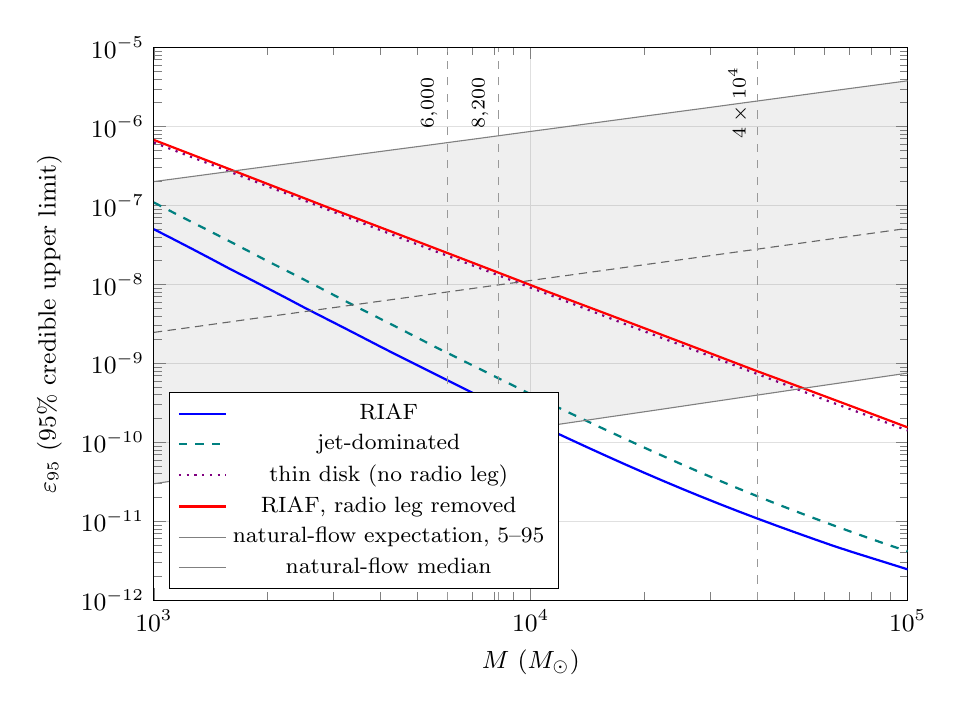
\begin{tikzpicture}
\begin{loglogaxis}[
  width=0.92\linewidth, height=8.6cm,
  xlabel={$M\ (\msun)$}, ylabel={$\epsl$ (95\% credible upper limit)},
  xmin=1000, xmax=100000, ymin=1e-12, ymax=1e-5,
  legend style={font=\footnotesize, at={(0.02,0.02)}, anchor=south west},
  grid=major, grid style={black!12},
  tick label style={font=\small}, label style={font=\small},
]
\addplot[blue, thick] coordinates {(1000,4.998e-08) (1122.02,3.775e-08) (1258.93,2.840e-08) (1412.54,2.128e-08) (1584.89,1.587e-08) (1778.28,1.199e-08) (1995.26,9.026e-09) (2238.72,6.773e-09) (2511.89,5.062e-09) (2818.38,3.824e-09) (3162.28,2.890e-09) (3548.13,2.178e-09) (3981.07,1.638e-09) (4466.84,1.237e-09) (5011.87,9.408e-10) (5623.41,7.152e-10) (6309.57,5.434e-10) (7079.46,4.127e-10) (7943.28,3.142e-10) (8912.51,2.418e-10) (10000,1.864e-10) (11220.2,1.439e-10) (12589.3,1.113e-10) (14125.4,8.640e-11) (15848.9,6.728e-11) (17782.8,5.261e-11) (19952.6,4.132e-11) (22387.2,3.262e-11) (25118.9,2.589e-11) (28183.8,2.066e-11) (31622.8,1.659e-11) (35481.3,1.339e-11) (39810.7,1.087e-11) (44668.4,8.867e-12) (50118.7,7.265e-12) (56234.1,5.975e-12) (63095.7,4.929e-12) (70794.6,4.114e-12) (79432.8,3.464e-12) (89125.1,2.917e-12) (100000,2.456e-12)};
\addlegendentry{RIAF}
\addplot[teal, thick, dashed] coordinates {(1000,1.091e-07) (1122.02,8.201e-08) (1258.93,6.180e-08) (1412.54,4.681e-08) (1584.89,3.533e-08) (1778.28,2.656e-08) (1995.26,1.990e-08) (2238.72,1.508e-08) (2511.89,1.139e-08) (2818.38,8.577e-09) (3162.28,6.436e-09) (3548.13,4.863e-09) (3981.07,3.685e-09) (4466.84,2.787e-09) (5011.87,2.102e-09) (5623.41,1.583e-09) (6309.57,1.207e-09) (7079.46,9.193e-10) (7943.28,6.998e-10) (8912.51,5.325e-10) (10000,4.052e-10) (11220.2,3.105e-10) (12589.3,2.393e-10) (14125.4,1.848e-10) (15848.9,1.429e-10) (17782.8,1.108e-10) (19952.6,8.615e-11) (22387.2,6.722e-11) (25118.9,5.266e-11) (28183.8,4.145e-11) (31622.8,3.278e-11) (35481.3,2.606e-11) (39810.7,2.083e-11) (44668.4,1.674e-11) (50118.7,1.353e-11) (56234.1,1.099e-11) (63095.7,8.966e-12) (70794.6,7.346e-12) (79432.8,6.040e-12) (89125.1,4.980e-12) (100000,4.171e-12)};
\addlegendentry{jet-dominated}
\addplot[violet, thick, dotted] coordinates {(1000,6.269e-07) (1122.02,5.067e-07) (1258.93,4.104e-07) (1412.54,3.323e-07) (1584.89,2.689e-07) (1778.28,2.176e-07) (1995.26,1.760e-07) (2238.72,1.423e-07) (2511.89,1.150e-07) (2818.38,9.292e-08) (3162.28,7.506e-08) (3548.13,6.062e-08) (3981.07,4.894e-08) (4466.84,3.951e-08) (5011.87,3.198e-08) (5623.41,2.595e-08) (6309.57,2.105e-08) (7079.46,1.707e-08) (7943.28,1.384e-08) (8912.51,1.121e-08) (10000,9.080e-09) (11220.2,7.351e-09) (12589.3,5.949e-09) (14125.4,4.813e-09) (15848.9,3.893e-09) (17782.8,3.147e-09) (19952.6,2.557e-09) (22387.2,2.080e-09) (25118.9,1.692e-09) (28183.8,1.375e-09) (31622.8,1.117e-09) (35481.3,9.067e-10) (39810.7,7.358e-10) (44668.4,5.969e-10) (50118.7,4.840e-10) (56234.1,3.922e-10) (63095.7,3.184e-10) (70794.6,2.600e-10) (79432.8,2.122e-10) (89125.1,1.730e-10) (100000,1.410e-10)};
\addlegendentry{thin disk (no radio leg)}
\addplot[red, thick] coordinates {(1000,6.758e-07) (1122.02,5.468e-07) (1258.93,4.423e-07) (1412.54,3.576e-07) (1584.89,2.891e-07) (1778.28,2.336e-07) (1995.26,1.887e-07) (2238.72,1.524e-07) (2511.89,1.231e-07) (2818.38,9.933e-08) (3162.28,8.044e-08) (3548.13,6.528e-08) (3981.07,5.295e-08) (4466.84,4.293e-08) (5011.87,3.480e-08) (5623.41,2.819e-08) (6309.57,2.283e-08) (7079.46,1.848e-08) (7943.28,1.496e-08) (8912.51,1.210e-08) (10000,9.784e-09) (11220.2,7.910e-09) (12589.3,6.427e-09) (14125.4,5.228e-09) (15848.9,4.250e-09) (17782.8,3.453e-09) (19952.6,2.804e-09) (22387.2,2.276e-09) (25118.9,1.847e-09) (28183.8,1.498e-09) (31622.8,1.214e-09) (35481.3,9.838e-10) (39810.7,7.980e-10) (44668.4,6.513e-10) (50118.7,5.312e-10) (56234.1,4.330e-10) (63095.7,3.527e-10) (70794.6,2.871e-10) (79432.8,2.336e-10) (89125.1,1.899e-10) (100000,1.543e-10)};
\addlegendentry{RIAF, radio leg removed}
\addplot[name path=n95, black!50, thin] coordinates {(1000,2.005e-07) (1122.02,2.156e-07) (1258.93,2.321e-07) (1412.54,2.498e-07) (1584.89,2.688e-07) (1778.28,2.893e-07) (1995.26,3.111e-07) (2238.72,3.345e-07) (2511.89,3.601e-07) (2818.38,3.868e-07) (3162.28,4.163e-07) (3548.13,4.477e-07) (3981.07,4.814e-07) (4466.84,5.178e-07) (5011.87,5.564e-07) (5623.41,5.985e-07) (6309.57,6.447e-07) (7079.46,6.932e-07) (7943.28,7.467e-07) (8912.51,8.043e-07) (10000,8.662e-07) (11220.2,9.313e-07) (12589.3,1.003e-06) (14125.4,1.080e-06) (15848.9,1.163e-06) (17782.8,1.252e-06) (19952.6,1.348e-06) (22387.2,1.450e-06) (25118.9,1.561e-06) (28183.8,1.679e-06) (31622.8,1.808e-06) (35481.3,1.949e-06) (39810.7,2.098e-06) (44668.4,2.260e-06) (50118.7,2.434e-06) (56234.1,2.623e-06) (63095.7,2.827e-06) (70794.6,3.042e-06) (79432.8,3.274e-06) (89125.1,3.522e-06) (100000,3.792e-06)};
\addlegendentry{natural-flow expectation, 5--95}
\addplot[name path=n05, black!50, thin] coordinates {(1000,2.985e-11) (1122.02,3.236e-11) (1258.93,3.508e-11) (1412.54,3.800e-11) (1584.89,4.120e-11) (1778.28,4.470e-11) (1995.26,4.848e-11) (2238.72,5.258e-11) (2511.89,5.700e-11) (2818.38,6.172e-11) (3162.28,6.684e-11) (3548.13,7.246e-11) (3981.07,7.861e-11) (4466.84,8.516e-11) (5011.87,9.233e-11) (5623.41,1.001e-10) (6309.57,1.087e-10) (7079.46,1.178e-10) (7943.28,1.276e-10) (8912.51,1.382e-10) (10000,1.500e-10) (11220.2,1.624e-10) (12589.3,1.760e-10) (14125.4,1.907e-10) (15848.9,2.069e-10) (17782.8,2.240e-10) (19952.6,2.428e-10) (22387.2,2.632e-10) (25118.9,2.855e-10) (28183.8,3.098e-10) (31622.8,3.358e-10) (35481.3,3.643e-10) (39810.7,3.952e-10) (44668.4,4.283e-10) (50118.7,4.648e-10) (56234.1,5.037e-10) (63095.7,5.457e-10) (70794.6,5.908e-10) (79432.8,6.404e-10) (89125.1,6.942e-10) (100000,7.518e-10)};
\addplot[black!60, fill opacity=0.10] fill between[of=n95 and n05];
\addplot[black!60, densely dashed] coordinates {(1000,2.465e-09) (1122.02,2.658e-09) (1258.93,2.864e-09) (1412.54,3.093e-09) (1584.89,3.338e-09) (1778.28,3.607e-09) (1995.26,3.887e-09) (2238.72,4.191e-09) (2511.89,4.519e-09) (2818.38,4.876e-09) (3162.28,5.255e-09) (3548.13,5.672e-09) (3981.07,6.119e-09) (4466.84,6.596e-09) (5011.87,7.109e-09) (5623.41,7.672e-09) (6309.57,8.278e-09) (7079.46,8.930e-09) (7943.28,9.643e-09) (8912.51,1.039e-08) (10000,1.121e-08) (11220.2,1.210e-08) (12589.3,1.304e-08) (14125.4,1.408e-08) (15848.9,1.519e-08) (17782.8,1.640e-08) (19952.6,1.770e-08) (22387.2,1.910e-08) (25118.9,2.060e-08) (28183.8,2.221e-08) (31622.8,2.397e-08) (35481.3,2.586e-08) (39810.7,2.789e-08) (44668.4,3.010e-08) (50118.7,3.246e-08) (56234.1,3.503e-08) (63095.7,3.781e-08) (70794.6,4.080e-08) (79432.8,4.403e-08) (89125.1,4.753e-08) (100000,5.127e-08)};
\addlegendentry{natural-flow median}
\draw[black!40, dashed] (axis cs:6000,1e-12) -- (axis cs:6000,1e-5);
\draw[black!40, dashed] (axis cs:8200,1e-12) -- (axis cs:8200,1e-5);
\draw[black!40, dashed] (axis cs:40000,1e-12) -- (axis cs:40000,1e-5);
\node[font=\scriptsize, rotate=90, anchor=south] at (axis cs:6000,2e-6) {$6{,}000$};
\node[font=\scriptsize, rotate=90, anchor=south] at (axis cs:8200,2e-6) {$8{,}200$};
\node[font=\scriptsize, rotate=90, anchor=south] at (axis cs:40000,2e-6) {$4\times10^{4}$};
\end{loglogaxis}
\end{tikzpicture}
\caption{95\,per~cent credible upper limits on the Bondi radiative efficiency $\eps$ of any central accretion flow in \ocen, per accretion-flow family, with the expectation band for a natural outflow-suppressed hot flow (grey: 5--95 percentile of $\varepsilon_{\mathrm{nat}} = \eta_{\mathrm{ADAF}}(\dot{m})\,f_{\mathrm{B}}$ over the same nuisance draws, on the \citet{XieYuan2012} efficiency of \S\ref{sec:eta}) rising while the limits fall. The band now sits above the RIAF limit across the whole range rather than crossing it inside the contested masses, which is why the exclusion fractions of Table~\ref{tab:anchors} are high at every anchor; the vertical separation is not itself the exclusion fraction, which \S\ref{sec:pexcl} defines from the likelihood rather than from this figure. Drafts to v1.5 drew this band two decades lower, on an efficiency linear in $\dot{m}$. Vertical lines mark the pulsar-timing point-mass cap \citep{BanaresHernandez2025}, the fast-star lower bound \citep{Haberle2024Nature}, and the upper kinematic range. All curves conditional on the $n_{e}$ prior of Table~\ref{tab:priors}.}
\label{fig:curves}
\end{figure}

Figure~\ref{fig:postcornerF} shows the full joint posterior behind these curves over the two parameters of interest and the two dominant nuisances, RIAF family only.

\begin{figure}[tbp]
\centering
\includegraphics[width=0.9\textwidth]{figs/fF_posterior_corner_v2.pdf}
\caption{Joint posterior corner plot for the RIAF family over the two parameters of interest ($\log_{10}\varepsilon_{95}$, the Bondi efficiency whose 95 per cent credible upper limit Figure~\ref{fig:curves} reports, and $\log_{10} M$) and the two dominant nuisances ($\log_{10} n_e$ and the distance). Samples from the shipped Monte Carlo (same seed, priors, and likelihood; $\eps$ log-uniform over the efficiency grid, per-sample weights $e^{\ln L}$; effective sample size $1.05\times10^{5}$ of $4\times10^{5}$ draws; script \texttt{figs/fF\_corner\_plot\_v2.py}). This figure alone adds a prior on $M$, log-uniform over the mass grid's range, because a corner plot needs a joint sample and the rest of the paper deliberately reports $\epsl$ at fixed $M$ instead of marginalizing over a mass prior the kinematic literature does not agree on. The $M$ panel therefore shows what that particular choice implies and is not a result of the paper. Contours enclose 68 and 90 per cent of the posterior weight. The $\eps$--$M$ degeneracy is the flux-limit constraint: the predicted X-ray, infrared, and radio luminosities all scale as $\eps\,M^{2}$ (Bondi) or steeper, so the posterior's upper envelope in $\eps$ falls as $M$ rises, the same structure Figure~\ref{fig:curves} displays curve by curve. The distance posterior reproduces its prior: the limits are flux measurements, and the drawn distance enters the prediction rather than the limit.}
\label{fig:postcornerF}
\end{figure}

\begin{table}[tbp]
\centering
\small
\caption{$\epsl$ at the three mass anchors (evaluated at the anchor masses, not grid neighbours), and the posterior-predictive exclusion fraction $P_{\mathrm{excl}}$ of \S\ref{sec:pexcl}: the fraction of natural-flow draws whose own predicted observables the measured data reject at the 5\,per~cent level. Monte Carlo standard errors on $P_{\mathrm{excl}}$ are below 0.003 throughout. The last column is the prior-exceedance fraction that drafts to v1.5 reported under the name $P_{\mathrm{excl}}$, recomputed here on independent draws.}
\label{tab:anchors}
\begin{tabular}{lcccccc}
\toprule
$M$ ($\msun$) & RIAF & jet & thin disk & RIAF, no radio & $P_{\mathrm{excl}}$ (RIAF) & prior exc. (RIAF) \\
\midrule
$6{,}000$ & $6.1\times10^{-10}$ & $1.4\times10^{-9}$ & $2.3\times10^{-8}$ & $2.5\times10^{-8}$ & 0.78 & 0.82 \\
$8{,}200$ & $2.9\times10^{-10}$ & $6.5\times10^{-10}$ & $1.3\times10^{-8}$ & $1.4\times10^{-8}$ & 0.85 & 0.89 \\
$4\times10^{4}$ & $1.1\times10^{-11}$ & $2.1\times10^{-11}$ & $7.3\times10^{-10}$ & $7.9\times10^{-10}$ & 0.99 & 1.00 \\
\bottomrule
\end{tabular}
\end{table}

Figure~\ref{fig:curves} and Table~\ref{tab:anchors} carry the content. Three statements summarize them.

\emph{The radio leg dominates wherever the fundamental plane applies.} The plane's mass term rises as $M^{0.78}$ while the Bondi denominator rises as $M^{2}$, which sets the direction; the realized slope of the marginalized limit is shallower than that single-draw asymptote, $\epsl \propto M^{-2.1}$ between the two upper anchors and $M^{-2.2}$ fitted across the whole grid, because the plane's 0.88-dex scatter and the two flux legs flatten the response. Drafts to v1.5 quoted the asymptote itself, $M^{-3.3}$, as though it were the realized slope. The radio-driven curve separates from the radio-free curve by 1.9 decades at the top of the mass range. This is the single-object version of the population-level result of \citet{Maccarone2005}, \citet{Strader2012}, and \citet{Tremou2018}: for IMBH masses, radio provides the tightest constraint on quiescent accretion. The plane's extrapolation into deep quiescence is contested \citep{Plotkin2012}, its 0.88-dex scatter is carried as a latent variable rather than a point estimate, and readers who distrust it entirely should quote the red curve: $\epsl = 1.4\times10^{-8}$ at $8{,}200\,\msun$ and $7.9\times10^{-10}$ at $4\times10^{4}\,\msun$, from Chandra and JWST with no shared emission model.

\emph{Against the natural-flow expectation, the verdict is no longer mass-dependent in the way earlier drafts reported.} The grey band is the prediction, $\varepsilon_{\mathrm{nat}} = \eta_{\mathrm{ADAF}}(\dot{m})\,f_{\mathrm{B}}$, evaluated draw by draw on the same nuisances, with $\eta_{\mathrm{ADAF}}$ now the piecewise fit of \citet{XieYuan2012} as summarized in \citet{YuanNarayan2014} and $\delta$ carried as a nuisance over the four values they tabulate (\S\ref{sec:eta}). This expectation carries no $\delta_{\mathrm{FP}}$ term, unlike \epsl{} for the RIAF and jet families, whose radio-leg prediction does (Section~\ref{sec:likelihood}); the fundamental-plane scatter widens the limit but not the band it is compared against, so a reader who distrusts the plane should read the exclusion fractions off the radio-free column rather than treating the asymmetry as a wash. The band rises with mass while every limit falls, and it now sits above the RIAF limit across the whole contested range rather than crossing inside it. At the pulsar-timing cap and the fast-star anchor the data reject 78 and 85\,per~cent of natural-flow draws under the RIAF family, and 20 and 28\,per~cent with the radio leg removed; at $4\times10^{4}\,\msun$ the figures are 99 and 76\,per~cent. Drafts to v1.5 reported 19, 31 and 90\,per~cent for the RIAF column, on a linear efficiency law and a statistic that compared the natural draws against a scalar built from those same draws; both are corrected here, and both corrections move the verdict the same way. Table~\ref{tab:sensexcl} carries the figures across the sensitivity ladder. A Bondi-fed hot flow at the fiducial density is now disfavoured across the contested mass range and not only at its top, which is a stronger claim than the one the earlier drafts made and a more fragile one, since it rests on extrapolating a published efficiency fit well below the rates it was computed for. Section~\ref{sec:eta} states what that extrapolation is worth and Table~\ref{tab:sensexcl}'s last two rows bracket it.

\emph{The thin disk is dead everywhere.} $\epsl$ for the disk family sits four to five decades below the $\eta \sim 0.06$--$0.4$ a disk radiates at; no Bondi-fed thin disk at any mass in the range survives, quantifying what every prior single-band paper assumed informally.

\subsection{The exclusion fraction as a continuous function of mass}
\label{sec:exclcurve}

Table~\ref{tab:anchors} evaluates $P_{\mathrm{excl}}$ at three masses because those are the masses the kinematic literature argues about. The Monte Carlo evaluates it on the whole grid, and the continuous version (Figure~\ref{fig:exclcurve}) is the more useful object for a reader who holds a different mass prior than any of the three anchors. It also locates the transitions. Under the RIAF family the exclusion fraction passes 50\,per~cent at $2.5\times10^{3}\,\msun$ and 90\,per~cent at $1.1\times10^{4}\,\msun$; under the jet family the same thresholds fall at $3.3\times10^{3}$ and $1.4\times10^{4}\,\msun$. Using no radio information they move to $1.7\times10^{4}$ and $7.9\times10^{4}\,\msun$. Both RIAF thresholds now sit below the pulsar-timing point-mass cap, so the mass-dependence that drafts to v1.5 built the verdict on has largely gone: on the corrected efficiency law the constraint bites across the contested range rather than only at its top.

\begin{figure}[tbp]
\centering
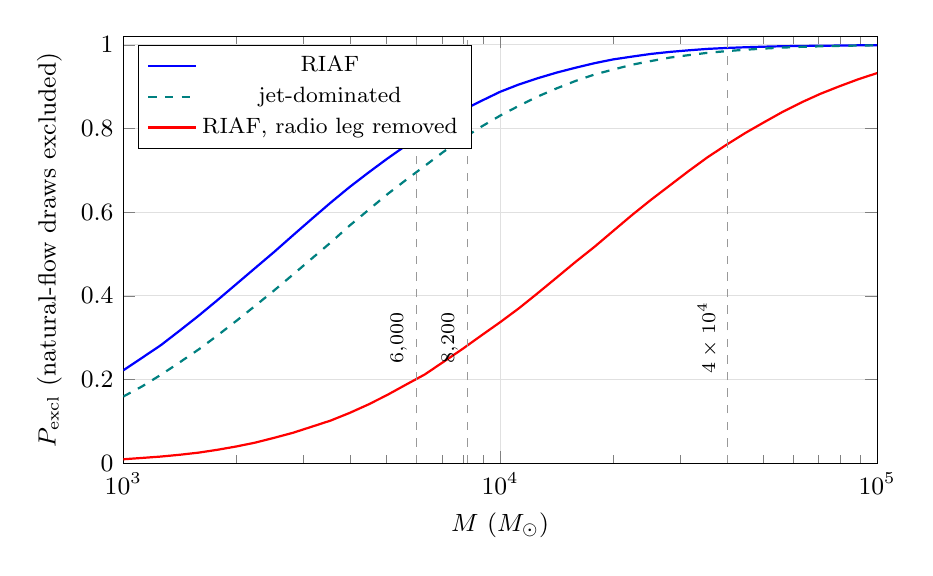
\begin{tikzpicture}
\begin{semilogxaxis}[
  width=0.92\linewidth, height=7.0cm,
  xlabel={$M\ (\msun)$}, ylabel={$P_{\mathrm{excl}}$ (natural-flow draws excluded)},
  xmin=1000, xmax=100000, ymin=0, ymax=1.02,
  legend style={font=\footnotesize, at={(0.02,0.98)}, anchor=north west},
  grid=major, grid style={black!12},
  tick label style={font=\small}, label style={font=\small},
]
\addplot[blue, thick] coordinates {(1000,0.2220) (1122.02,0.2521) (1258.93,0.2824) (1412.54,0.3172) (1584.89,0.3527) (1778.28,0.3900) (1995.26,0.4283) (2238.72,0.4667) (2511.89,0.5049) (2818.38,0.5447) (3162.28,0.5840) (3548.13,0.6228) (3981.07,0.6599) (4466.84,0.6945) (5011.87,0.7279) (5623.41,0.7595) (6309.57,0.7891) (7079.46,0.8173) (7943.28,0.8435) (8912.51,0.8662) (10000,0.8880) (11220.2,0.9056) (12589.3,0.9205) (14125.4,0.9339) (15848.9,0.9455) (17782.8,0.9563) (19952.6,0.9654) (22387.2,0.9721) (25118.9,0.9785) (28183.8,0.9833) (31622.8,0.9871) (35481.3,0.9905) (39810.7,0.9927) (44668.4,0.9944) (50118.7,0.9958) (56234.1,0.9969) (63095.7,0.9976) (70794.6,0.9980) (79432.8,0.9985) (89125.1,0.9990) (100000,0.9994)};
\addlegendentry{RIAF}
\addplot[teal, thick, dashed] coordinates {(1000,0.1594) (1122.02,0.1837) (1258.93,0.2115) (1412.54,0.2414) (1584.89,0.2720) (1778.28,0.3055) (1995.26,0.3403) (2238.72,0.3764) (2511.89,0.4129) (2818.38,0.4508) (3162.28,0.4892) (3548.13,0.5274) (3981.07,0.5677) (4466.84,0.6051) (5011.87,0.6426) (5623.41,0.6772) (6309.57,0.7108) (7079.46,0.7448) (7943.28,0.7757) (8912.51,0.8046) (10000,0.8310) (11220.2,0.8546) (12589.3,0.8768) (14125.4,0.8962) (15848.9,0.9139) (17782.8,0.9292) (19952.6,0.9412) (22387.2,0.9527) (25118.9,0.9615) (28183.8,0.9697) (31622.8,0.9756) (35481.3,0.9811) (39810.7,0.9851) (44668.4,0.9885) (50118.7,0.9913) (56234.1,0.9936) (63095.7,0.9955) (70794.6,0.9967) (79432.8,0.9977) (89125.1,0.9985) (100000,0.9991)};
\addlegendentry{jet-dominated}
\addplot[red, thick] coordinates {(1000,0.0094) (1122.02,0.0126) (1258.93,0.0159) (1412.54,0.0202) (1584.89,0.0253) (1778.28,0.0321) (1995.26,0.0400) (2238.72,0.0492) (2511.89,0.0606) (2818.38,0.0727) (3162.28,0.0872) (3548.13,0.1019) (3981.07,0.1200) (4466.84,0.1403) (5011.87,0.1630) (5623.41,0.1878) (6309.57,0.2122) (7079.46,0.2426) (7943.28,0.2731) (8912.51,0.3054) (10000,0.3372) (11220.2,0.3706) (12589.3,0.4069) (14125.4,0.4440) (15848.9,0.4814) (17782.8,0.5172) (19952.6,0.5554) (22387.2,0.5935) (25118.9,0.6297) (28183.8,0.6641) (31622.8,0.6985) (35481.3,0.7314) (39810.7,0.7611) (44668.4,0.7893) (50118.7,0.8151) (56234.1,0.8403) (63095.7,0.8629) (70794.6,0.8833) (79432.8,0.9011) (89125.1,0.9179) (100000,0.9327)};
\addlegendentry{RIAF, radio leg removed}
\draw[black!40, dashed] (axis cs:6000,0) -- (axis cs:6000,1.02);
\draw[black!40, dashed] (axis cs:8200,0) -- (axis cs:8200,1.02);
\draw[black!40, dashed] (axis cs:40000,0) -- (axis cs:40000,1.02);
\node[font=\scriptsize, rotate=90, anchor=south] at (axis cs:6000,0.30) {$6{,}000$};
\node[font=\scriptsize, rotate=90, anchor=south] at (axis cs:8200,0.30) {$8{,}200$};
\node[font=\scriptsize, rotate=90, anchor=south] at (axis cs:40000,0.30) {$4\times10^{4}$};
\end{semilogxaxis}
\end{tikzpicture}
\caption{Fraction of natural-flow parameter space excluded, $P_{\mathrm{excl}}$ of Eq.~\ref{eq:pexcl}, as a continuous function of mass: every natural-flow draw scored against the measured data at every grid mass rather than at three. Drafts to v1.5 plotted the prior-exceedance fraction $P[\varepsilon_{\mathrm{nat}} > \epsl]$ here; that curve is carried alongside in the shipped output. Vertical lines mark the pulsar-timing point-mass cap \citep{BanaresHernandez2025}, the fast-star lower bound \citep{Haberle2024Nature}, and the upper kinematic range. The three anchor values of Table~\ref{tab:anchors} sit on these curves by construction. Coordinates from \texttt{figs/fF\_expand\_exclcurve\_v2.json}. The quantity plotted is the posterior-predictive fraction of \S\ref{sec:pexcl}; that file also carries the prior-exceedance curve the v1.5 figure plotted, so the change is auditable.}
\label{fig:exclcurve}
\end{figure}

\subsection{Which band binds which family}
\label{sec:bandadj}

Figure~\ref{fig:bands} shows what the family definitions of Section~\ref{sec:families} change. At each anchor the figure evaluates the forward model at that family's own $\epsl$ and plots the predicted $\nu L_{\nu}$ in every observed band against the published limit in that band, so the three instruments and the three families appear on one axis.

The radio leg binds every family that carries it, and by a wide margin. For the RIAF family the median predicted radio flux density at \epsl{} sits at 1.5 times the ATCA $5\sigma$ point at $8{,}200\,\msun$ and 4.8 times it at $4\times10^{4}\,\msun$, while the X-ray prediction sits at about 1\,per~cent of the Chandra bound and the tightest infrared filter at 0.2\,per~cent of its own. For the jet family, the one built to be infrared-bright, the radio ratios are 1.2 and 3.6 and the F770W ratio reaches 0.8 and 0.6\,per~cent: better than under the RIAF band fractions by a factor of five, and still short of the plane by more than two decades. Drafts to v1.5 described JWST as genuinely binding for this family. It does not, on their own numbers or these, and the correction of Section~\ref{sec:data} to the infrared comparison widens the gap rather than closing it.

The thin disk carries no radio leg, and there the X-ray band binds alone, at 0.43 and 0.58 of the Chandra bound against F770W's 0.09 and 0.12. Drafts to v1.5 reported those two legs sharing the constraint within 10\,per~cent of each other; that reading came from comparing a band-peak prediction against a band-integrated limit, and once the two are the same quantity the infrared sits a factor of five below the X-ray in every family. The honest summary is that this is a radio-plus-X-ray bound with an infrared consistency check, not a three-way joint constraint, and Section~\ref{sec:forecast} prices deeper mid-infrared accordingly.

Ratios above unity for the radio band are expected and are not a detection claim: $\epsl$ is a 95\,per~cent posterior quantile marginalized over the plane's 0.88-dex latent scatter, so at that $\eps$ the median draw predicts a flux the image would have seen while a substantial tail does not. The five-percentile whiskers, which reach two decades below the medians in the radio and a factor of ten in the other bands, are that scatter. The infrared points were flat across the four filters in drafts to v1.5, since the model predicts one band-peak $\nu L_{\nu}$ and the filters differed only in their limits. They are no longer flat: each is now converted to that filter's band-integrated luminosity by its own $\Delta\lambda/\lambda_{c}$ (Table~\ref{tab:irfilters}), which is the quantity the published limits are. F770W still sets the infrared constraint, by a factor of two over the next filter, because it combines the tightest limit with the narrowest fractional bandwidth.

\begin{figure}[tbp]
\centering
\includegraphics[width=\linewidth]{figs/fF_expand_sed_v2.png}
\caption{Predicted band luminosities at each family's own $\epsl$, against the published limits (black bars, arrows marking the excluded direction). Points are medians over the $4\times10^{4}$ nuisance draws, whiskers the 5th to 95th percentiles. The thin-disk family has no radio point because the fundamental-plane leg is not applied to it (Section~\ref{sec:families}). The radio limit is drawn at $5\sigma$ (5.5\,$\mu$Jy) so that it is comparable with the X-ray and infrared bounds, which are published as limits; the likelihood itself uses the $1.1\,\mu$Jy rms as a Gaussian $\sigma$ and is unaffected. Infrared points are band-integrated luminosities, the same quantity as the published limits (\S\ref{sec:data}); drafts to v1.5 plotted band-peak predictions against band-integrated limits here. Script \texttt{figs/fF\_expand\_v2.py}, numbers in \texttt{figs/fF\_expand\_sed\_v2.json}.}
\label{fig:bands}
\end{figure}

\subsection{Sensitivity budget}
\label{sec:sensitivity}

\begin{table}[tbp]
\centering
\small
\caption{Sensitivity of the RIAF-family \epsl{} to the dominant analysis choices. Each row changes one ingredient from the baseline.}
\label{tab:sens}
\begin{tabular}{lccc}
\toprule
Variant & $6{,}000\,\msun$ & $8{,}200\,\msun$ & $4\times10^{4}\,\msun$ \\
\midrule
baseline & $6.1\times10^{-10}$ & $2.9\times10^{-10}$ & $1.1\times10^{-11}$ \\
$n_{e}$ prior widened to 1.5\,dex & $3.5\times10^{-9}$ & $1.7\times10^{-9}$ & $7.4\times10^{-11}$ \\
$n_{e}$ prior median $\div\,10$ & $3.7\times10^{-9}$ & $1.7\times10^{-9}$ & $4.4\times10^{-11}$ \\
widened + wind truncation ($n_{e} \geq 0.02$) & $1.0\times10^{-9}$ & $5.1\times10^{-10}$ & $1.8\times10^{-11}$ \\
widened + retired floor ($n_{e} \geq 0.05$) & $6.7\times10^{-10}$ & $3.3\times10^{-10}$ & $1.2\times10^{-11}$ \\
$\eps$-grid floor raised to $10^{-11}$ & $5.5\times10^{-9}$ & $3.3\times10^{-9}$ & $4.4\times10^{-10}$ \\
IR band correction removed (the v1.5 leg) & $5.7\times10^{-10}$ & $2.8\times10^{-10}$ & $1.0\times10^{-11}$ \\
$k$ at $\Gamma = 2.3$, the source's own index & $7.3\times10^{-10}$ & $3.5\times10^{-10}$ & $1.2\times10^{-11}$ \\
\bottomrule
\end{tabular}
\end{table}

\begin{table}[tbp]
\centering
\small
\caption{The posterior-predictive exclusion fraction under the same variants,
for the RIAF family and for the radio-free curve. Table~\ref{tab:sens} moves
only \epsl; here the natural-flow draws move with the nuisances, since both
are built from one set of draws. The $\eps$-grid floor has no row: the
statistic of \S\ref{sec:pexcl} never reads \epsl{}, so the efficiency prior's
lower cutoff cannot reach it, which is one practical gain of the
reconstruction. Monte Carlo standard errors are below 0.003 throughout.}
\label{tab:sensexcl}
\begin{tabular}{lcccccc}
\toprule
& \multicolumn{3}{c}{RIAF} & \multicolumn{3}{c}{RIAF, no radio} \\
\cmidrule(lr){2-4}\cmidrule(lr){5-7}
Variant & $6{,}000$ & $8{,}200$ & $4{\times}10^{4}$ & $6{,}000$ & $8{,}200$ & $4{\times}10^{4}$ \\
\midrule
baseline & 0.78 & 0.85 & 0.99 & 0.20 & 0.28 & 0.76 \\
$n_{e}$ prior widened to 1.5\,dex & 0.69 & 0.75 & 0.94 & 0.33 & 0.38 & 0.64 \\
$n_{e}$ prior median $\div\,10$ & 0.47 & 0.58 & 0.94 & 0.02 & 0.04 & 0.33 \\
widened + wind truncation ($n_{e} \geq 0.02$) & 0.74 & 0.81 & 0.98 & 0.33 & 0.38 & 0.69 \\
widened + retired floor ($n_{e} \geq 0.05$) & 0.79 & 0.85 & 0.99 & 0.34 & 0.40 & 0.75 \\
X-ray limit read two-sided 95\,per~cent & 0.78 & 0.85 & 0.99 & 0.21 & 0.30 & 0.78 \\
X-ray limit read as $3\sigma$ & 0.78 & 0.85 & 0.99 & 0.25 & 0.34 & 0.81 \\
$k$ at $\Gamma = 2.3$ & 0.76 & 0.84 & 0.99 & 0.20 & 0.28 & 0.76 \\
IR completeness row 99.7\,per~cent & 0.78 & 0.85 & 0.99 & 0.20 & 0.28 & 0.76 \\
IR completeness row 68\,per~cent & 0.78 & 0.85 & 0.99 & 0.21 & 0.29 & 0.77 \\
IR tightest single filter only & 0.80 & 0.87 & 0.99 & 0.23 & 0.31 & 0.79 \\
IR band correction removed (the v1.5 leg) & 0.78 & 0.85 & 0.99 & 0.25 & 0.33 & 0.81 \\
Bondi denominator, Paper~E convention & 0.73 & 0.82 & 0.99 & 0.15 & 0.22 & 0.70 \\
\midrule
$\eta$ held at the XY12 fit's own lower edge & 0.99 & 1.00 & 1.00 & 0.87 & 0.92 & 1.00 \\
$\eta$ linear in $\dot{m}$ (the v1.5 form) & 0.36 & 0.48 & 0.92 & 0.01 & 0.02 & 0.27 \\
\bottomrule
\end{tabular}
\end{table}

Table~\ref{tab:sensexcl} prices the headline verdict rather than the limit
behind it, and the two no longer move together in the way drafts to v1.5
described. Widening the $n_{e}$ prior costs the RIAF exclusion fraction 0.09
at the fast-star anchor and 0.05 at the high anchor; shifting the prior centre
down a decade costs 0.27 at the fast-star anchor while leaving the high anchor
at 0.94, because at $4\times10^{4}\,\msun$ the natural-flow band clears the
limit by enough margin that a factor of ten in density does not close it. The
prior-shift row is still the widest single move, and \S\ref{sec:gas}'s recount
is an argument that it is the more likely direction rather than a worst case.
Across every convention choice in this paper the RIAF exclusion fraction at
$4\times10^{4}\,\msun$ stays above 0.93 and at $8{,}200\,\msun$ above 0.57;
the radio-free column is the fragile one, spanning 0.02 to 0.40 at the
fast-star anchor and 0.33 to 0.81 at the high anchor, and it should be read
with that range attached. Two rows below the rule price the efficiency
prescription itself rather than a convention: holding $\eta$ at the lower edge
of the range Xie \& Yuan actually computed, instead of extrapolating their fit
four to six decades below it, raises every entry towards unity, while the
linear $\eta$ of drafts to v1.5 lowers them to the values those drafts
reported. The extrapolation this paper adopts is the weaker of the two
readings of the cited fit, and the verdict is stated on that reading.

Table~\ref{tab:sens} is the quantified version of Section~\ref{sec:priors}'s caveat. Widening the $n_{e}$ prior by a decade in each direction, or dividing its median by ten, each relax \epsl{} by a factor of about six: the curve's normalization belongs to the gas-density assumption, in both its width and its centre, and no claim in this paper escapes that conditioning. The damage is bounded on one side and, since v1.5, no longer on the other. Truncating the widened prior at $n_{e} \geq 0.02\,\mathrm{cm^{-3}}$, inside the range the wind recount of Section~\ref{sec:gas} supports, recovers about two thirds of the widening in the log: \epsl{} at the fast-star anchor moves from $1.7\times10^{-9}$ back to $5.1\times10^{-10}$ against a baseline of $2.9\times10^{-10}$. Drafts to v1.5 used a truncation at $0.05\,\mathrm{cm^{-3}}$ and reported that it returned the widened prior almost to baseline; that floor lies above the wind steady state and the claim is withdrawn with it. The $\eps$-prior floor matters as it always does for non-detections, by a factor of 9 at the two lower anchors and 40 at $4\times10^{4}\,\msun$ when the grid floor rises three decades; drafts to v1.5 quoted that as a single factor of about ten, which holds only at the lower anchors. Every \epsl{} here is quoted on the $10^{-14}$ grid, the machine-readable likelihood tables let any reader impose their own, and the exclusion fractions of Table~\ref{tab:sensexcl} are now independent of that choice entirely.

\subsubsection{Which nuisance carries the spread}
\label{sec:nuisance}

Table~\ref{tab:sens} varies analysis choices. The nuisance parameters can be interrogated separately, by re-running the same posterior with one of them held at its prior's central value while the others are drawn, and again with only that one drawn and the others held (Figure~\ref{fig:nuisance}). The two views answer different questions: the first asks how much of the limit's looseness a given parameter is responsible for, the second asks how much looseness that parameter would produce on its own. Seven parameters appear; the eighth, $\delta$, is absent for the same structural reason as $s$, since it enters $\varepsilon_{\mathrm{nat}}$ and not the likelihood, so freezing it cannot move \epsl.

The answer is that the fundamental plane's latent scatter carries the spread. Freezing $\delta_{\mathrm{FP}}$ at zero tightens \epsl{} by a factor of 13 at $8{,}200\,\msun$ and 29 at $4\times10^{4}\,\msun$; drawing it alone, with everything else fixed, reproduces a limit 18 and 61 times looser than the fully frozen case. No other parameter comes within an order of magnitude. The gas density is second and is a distant second in this accounting: freezing it tightens \epsl{} by 21 to 25\,per~cent, and drawing it alone loosens the frozen limit by a factor 1.6 to 2.4. The X-ray band fraction contributes 8 to 10\,per~cent, the sound speed under 1\,per~cent, and the distance nothing measurable, as expected from a 1\,per~cent prior. The infrared band fraction moves the RIAF limit by 0.4\,per~cent in the opposite direction, which is the signature of a leg that never binds in this family, and the band correction of Section~\ref{sec:data} makes it smaller still than the 2\,per~cent drafts to v1.5 reported.

The distance prior and the suppression index are inert here, for structural reasons worth naming. The distance prior is narrow enough that its 1\,per~cent width cannot register against the plane's 0.88 dex. The suppression index $s$ does not enter the likelihood at all: it sets the natural-flow expectation $\varepsilon_{\mathrm{nat}}$ against which the limit is compared, not the limit itself, so its entire influence in this paper runs through $P_{\mathrm{excl}}$ and the grey band of Figure~\ref{fig:curves} rather than through \epsl.

This does not contradict Section~\ref{sec:priors}'s statement that the gas density owns the result. The two statements are about different things. Within the stated priors, the plane's scatter is what widens the posterior; the density's danger is in the choice of prior centre, which no freezing test can expose, and which Table~\ref{tab:sens}'s prior-shift rows price at a factor $\sim$6. A reader who distrusts the plane has the radio-free curve; a reader who distrusts the density analogy has the shift rows and the wind recount of Section~\ref{sec:gas}, which points the same way.

\begin{figure}[tbp]
\centering
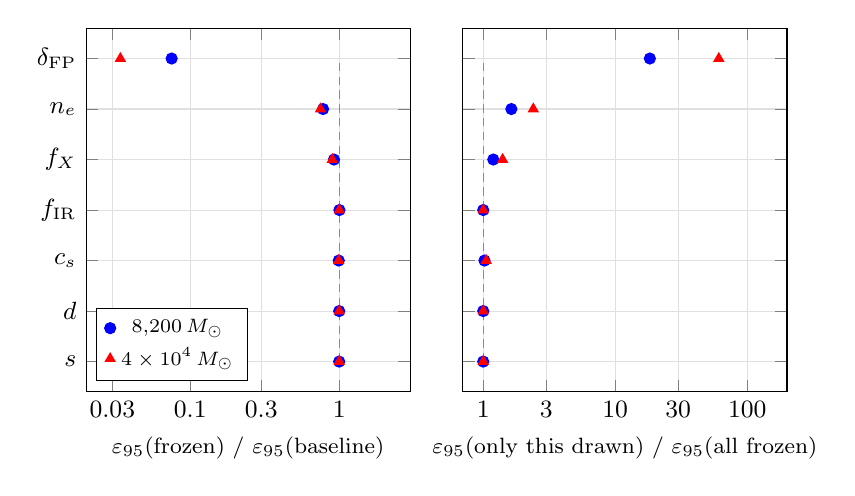
\begin{tikzpicture}
\begin{semilogxaxis}[
  width=0.47\linewidth, height=6.2cm,
  name=leftplot,
  xlabel={$\epsl$(frozen) / $\epsl$(baseline)},
  xmin=0.02, xmax=3, xtick={0.03,0.1,0.3,1},
  xticklabels={0.03,0.1,0.3,1},
  ytick=data, symbolic y coords={s,d,c_s,f_IR,f_X,n_e,fp},
  yticklabels={$s$,$d$,$c_{s}$,$f_{\mathrm{IR}}$,$f_{X}$,$n_{e}$,$\delta_{\mathrm{FP}}$},
  grid=major, grid style={black!12},
  tick label style={font=\small}, label style={font=\footnotesize},
  legend style={font=\scriptsize, at={(0.03,0.03)}, anchor=south west},
]
\addplot[only marks, mark=*, blue] coordinates {(1.0000,s) (1.0000,d) (0.9937,c_s) (1.0036,f_IR) (0.9228,f_X) (0.7796,n_e) (0.0751,fp)};
\addlegendentry{$8{,}200\,\msun$}
\addplot[only marks, mark=triangle*, red] coordinates {(1.0000,s) (0.9999,d) (0.9931,c_s) (1.0022,f_IR) (0.8990,f_X) (0.7492,n_e) (0.0340,fp)};
\addlegendentry{$4\times10^{4}\,\msun$}
\draw[black!45, densely dashed] (axis cs:1,s) -- (axis cs:1,fp);
\end{semilogxaxis}
\begin{semilogxaxis}[
  width=0.47\linewidth, height=6.2cm,
  at={(leftplot.east)}, anchor=west, xshift=0.055\linewidth,
  xlabel={$\epsl$(only this drawn) / $\epsl$(all frozen)},
  xmin=0.7, xmax=200, xtick={1,3,10,30,100},
  xticklabels={1,3,10,30,100},
  ytick=data, symbolic y coords={s,d,c_s,f_IR,f_X,n_e,fp},
  yticklabels={,,,,,,},
  grid=major, grid style={black!12},
  tick label style={font=\small}, label style={font=\footnotesize},
]
\addplot[only marks, mark=*, blue] coordinates {(1.0000,s) (1.0000,d) (1.0220,c_s) (1.0000,f_IR) (1.1922,f_X) (1.6341,n_e) (18.2931,fp)};
\addplot[only marks, mark=triangle*, red] coordinates {(1.0000,s) (1.0004,d) (1.0530,c_s) (1.0000,f_IR) (1.4032,f_X) (2.3953,n_e) (60.9010,fp)};
\draw[black!45, densely dashed] (axis cs:1,s) -- (axis cs:1,fp);
\end{semilogxaxis}
\end{tikzpicture}
\caption{Per-nuisance contribution to the RIAF-family limit, at two mass anchors. Left: \epsl{} with that nuisance held at its prior's central value, divided by the baseline \epsl{}; a point far to the left means that parameter's spread was inflating the limit by that factor. Right: \epsl{} with only that nuisance drawn, divided by the limit with all seven frozen. Neither panel is a variance decomposition, since \epsl{} is a posterior quantile rather than a sum of independent terms, and the two panels do not multiply back to unity. The distance and the suppression index sit on the reference line in both panels; $s$ does so because it enters the natural-flow expectation and not the likelihood. Numbers in \texttt{figs/fF\_expand\_nuisance\_v2.json}.}
\label{fig:nuisance}
\end{figure}

\subsection{Where this sits against the survey population}
\label{sec:maveric}

The single-cluster depth used here is best read against the 50-cluster MAVERIC survey \citep{Tremou2018}, which is the reference population for radio IMBH limits and the source of the field's null (Table~\ref{tab:maveric}). Two cautions travel with the comparison. First, each entry assumes its own distance: \citet{Tremou2018} adopt 4.9\,kpc for \ocen{}, \citet{Haggard2013} 5.2\,kpc, \citet{Chen2025JWST} and \citet{Mahida2026} 5.49\,kpc, against this paper's 5.43\,kpc prior. The spread is ordinary paper-to-paper variation and it propagates as $d^{2}$ into any luminosity, so the flux densities compare directly while the derived quantities do not. Second, the survey's mass limits are obtained by inverting the fundamental plane, the step Section~\ref{sec:likelihood} declines to take; they are quoted here as the literature's own currency and are not $\eps$ and not convertible to it without the full nuisance treatment.

\begin{table}[htbp]
\centering
\small
\caption{Radio limits on central sources in globular clusters, as published. Mass limits are the sources' own fundamental-plane inversions, quoted at $3\sigma$; they are not $\eps$. Flux densities are directly comparable, derived quantities are not.}
\label{tab:maveric}
\begin{tabular}{llll}
\toprule
Dataset & Depth & Derived limit & Assumed $d$ \\
\midrule
MAVERIC ATCA, \ocen{} \citep{Tremou2018} & $<8.8\,\mu$Jy ($3\sigma$) & $M < 1000\,\msun$ & 4.9\,kpc \\
MAVERIC VLA stack, 24 clusters & 0.65\,$\mu$Jy\,beam$^{-1}$ & $M < 800\,\msun$ & per cluster \\
MAVERIC ATCA stack, 14 clusters & 1.42\,$\mu$Jy\,beam$^{-1}$ & $M < 970\,\msun$ & per cluster \\
This paper's radio input \citep{Mahida2026} & 1.1\,$\mu$Jy\,beam$^{-1}$ rms & see Fig.~\ref{fig:curves} & 5.49\,kpc \\
\bottomrule
\end{tabular}
\end{table}

The ATCA campaign of \citet{Mahida2026} is deeper on one cluster than the MAVERIC stack is on 24, which is what makes a per-object posterior worth building at all. Three ambiguities in the survey paper are carried rather than resolved: its \ocen{} flux limit appears as 8.8\,$\mu$Jy in Table~2 and 8.9\,$\mu$Jy in Section~V.2.1; its VLA stack mass limit is given as both $<800$ and $<730\,\msun$ in a single sentence, and we quote the weaker; and whether \ocen{} enters the 14-cluster ATCA stack is not stated, though the paper's explicit exclusion list omits it. Its comparison of the \ocen{} radio limit against \citet{Haggard2013} also cites the X-ray limit as $1.7\times10^{30}\,\mathrm{erg\,s^{-1}}$ where \citeauthor{Haggard2013} state $1.6\times10^{30}$, which looks like a transcription rounding. None of this affects the numbers of Section~\ref{sec:results}, which use no MAVERIC input; it affects only what the reader should do with the row above.

\section{The duty-cycle loophole}
\label{sec:duty}

The three inputs sample time very differently, and \citet{Mahida2026}'s Table~1 makes the radio sampling explicit: 25 observing blocks across three ATCA projects, 2010 January 22 to 2024 December 27, summing to 177.19\,hr on source (CX556, 20 blocks, 147.09\,hr; C2877, 3 blocks, 11.79\,hr; C2158, 2 blocks, 18.31\,hr). Those rows exceed the $\sim$170\,hr of the paper's abstract and the 172\,hr of its Section~II.3; we report the sum as printed and leave the reconciliation to that paper, noting that prose totals quoted after flagging would run below a raw table sum rather than above it. Chandra contributes four exposures in two epochs twelve years apart, JWST a single epoch.

Two consequences follow on different timescales. For variability slower than the sampled span, the limits above apply to the time-average $\delta\,\varepsilon_{\mathrm{on}}$ of a flow active a fraction $\delta$ of the time at $\varepsilon_{\mathrm{on}}$, so $\varepsilon_{\mathrm{on}} \lesssim \epsl/\delta$; the radio image is a weighted combination over the full fourteen-year span, so this is the operative statement there. For variability faster than a block, the source must be off during every epoch to escape, which for $N \simeq 30$ independent epochs (25 radio blocks, four Chandra exposures, one JWST visit) gives a miss probability $(1-\delta)^{N}$ reaching 50\,per~cent only near $\delta \approx 0.02$. This order-of-magnitude estimate counts every block or exposure as one independent trial regardless of its duration relative to the assumed flare timescale $\tau$; Section~\ref{sec:dutyquant}'s block-by-block treatment does not carry that assumption and supersedes this estimate in rigor. The excluded region is therefore the band $\varepsilon_{\mathrm{on}} > \epsl/\delta$ down to a few per~cent duty cycle, and effectively nothing below that: a flow that spends 99\,per~cent of its time off is constrained only by the luck of the sampling. An earlier draft put the epoch count at $N \sim 6$ and the sampling break at $\delta \approx 0.1$, having treated the radio campaign as one epoch. This is the standard loophole of every quiescent-limit paper, here made explicit because Paper E's tidal-disruption arithmetic predicts exactly such intermittency on $10^{7}$-yr recurrence with $10^{-4}$ duty, far below the reach of any current sampling; nothing in this paper's nulls bears on that channel, in either direction.

\subsection{What the block list actually excludes}
\label{sec:dutyquant}

The block list supports a stronger statement than a miss probability, because each block is an image in its own right. Scaling the combined image's sensitivity by on-source time, $\sigma_{i} = 1.1\,\mu\mathrm{Jy}\,\sqrt{177.19\,\mathrm{hr}/t_{i}}$, the 25 blocks reach 4.5 to 12.0\,$\mu$Jy rms with a median of 5.3\,$\mu$Jy over a median 7.6\,hr on source, so a single block detects a source at $5\sigma$ near 27\,$\mu$Jy while the combined image reaches 5.5\,$\mu$Jy. That scaling assumes each on-source hour is equally sensitive across the three projects and both observing frequencies, which \citet{Mahida2026} do not state block by block; it is the only scaling their published table supports. The block statistics in this paragraph regenerate from \texttt{figs/fF\_epochs.json}, the export of that table: 25 blocks spanning 1.48 to 10.70\,hr on source, rms 4.48 to 12.04\,$\mu$Jy, median 5.31\,$\mu$Jy.

A flare train is then a two-parameter object: amplitude $S$ and duration $\tau$, recurring with period $T_{\mathrm{rec}}$ at an unknown phase. Laying such a train over the real block timeline (2010 January 22 to 2024 December 27, a 14.9-yr span containing 177.19\,hr of on-source time) and asking whether any single block's $\tau$-averaged flux exceeds its own $5\sigma$ point, or the campaign mean exceeds 5.5\,$\mu$Jy, gives a detection probability over phase. Table~\ref{tab:duty} reports, for each $(S, \tau)$, the longest recurrence interval that would still have been caught in at least 95\,per~cent of phases. Anything recurring faster than that is excluded; anything slower is not.

\begin{table}[tbp]
\centering
\small
\caption{Longest flare recurrence interval excluded at 95\,per~cent of phases,
from the 25-block ATCA timeline (4000 fixed-seed realizations per cell; script
\texttt{figs/fF\_expand\_v1.py}, seed 20260820). Entries are hours; a dash means
no recurrence interval on the grid is excluded for that amplitude and duration.
The implied duty cycle at each threshold, $\tau/T_{\mathrm{rec}}$ computed at the
unrounded threshold, is in parentheses; recomputing it from the rounded hours in
this table gives a value differing by up to 2\,per~cent. Thresholds are located
on a recurrence grid of 45 logarithmic points spanning 6\,hr to $2\times10^{5}$\,hr,
a 27\,per~cent step, which sets the precision of every entry.}
\label{tab:duty}
\begin{tabular}{lcccc}
\toprule
Flare amplitude & $\tau = 0.5$\,hr & 2\,hr & 8\,hr & 24\,hr \\
\midrule
$10\,\mu$Jy & -- & -- & $12$ (0.655) & $31$ (0.763) \\
$30\,\mu$Jy & -- & $8$ (0.263) & $25$ (0.322) & $130$ (0.184) \\
$100\,\mu$Jy & $8$ (0.066) & $31$ (0.064) & $130$ (0.061) & $209$ (0.115) \\
$300\,\mu$Jy & $15$ (0.032) & $81$ (0.025) & $130$ (0.061) & $209$ (0.115) \\
$1$\,mJy & $81$ (0.006) & $81$ (0.025) & $130$ (0.061) & $209$ (0.115) \\
\bottomrule
\end{tabular}
\end{table}

Low-amplitude trains are excluded only when they are almost always on: a 10\,$\mu$Jy source is invisible in any single block and can be caught only through the campaign mean, which requires a duty cycle above 0.7. Bright, brief trains are bounded by the sampling rather than by the sensitivity: at 300\,$\mu$Jy and above, for durations of 2\,hr and longer, the exclusion saturates near a recurrence interval of 3 to 9\,days, because 177\,hr of on-source time spread over 14.9\,yr covers 0.14\,per~cent of the span, and a flare that recurs more slowly than about a week simply misses every block most of the time no matter how bright it is. Between those regimes the campaign excludes real parameter space: a 100\,$\mu$Jy, 2-hr flare is excluded for recurrence faster than 31\,hr, a duty cycle of $6\times10^{-2}$.

The scaling's own uncertainty can be priced. Drawing per-block sensitivity
log-normally about it, at fixed combined campaign sensitivity, since the
1.1\,$\mu$Jy combined rms is measured rather than assumed, moves the table
where the single-block channel sets the threshold and leaves it alone where
the campaign mean does. At 0.2\,dex of scatter, two of the fourteen
well-determined cells move by one grid step: the $30\,\mu$Jy, 24-hr threshold
falls from 130 to 81\,hr and the $100\,\mu$Jy, 2-hr threshold from 31 to 25\,hr.
Both $10\,\mu$Jy rows hold to the digit at every scatter level tested, up to
0.3\,dex, because a $10\,\mu$Jy source is caught only through the campaign mean,
whose depth is measured. The floor of the excluded region is likewise
unaffected at $\pm$30\,per~cent per-block rms, and reaches a duty cycle of
$1\times10^{-2}$ only at 0.3\,dex. The caveat this paragraph opens with
therefore attaches to the mid-amplitude, long-duration cells rather than to the
faint end, which the source paper's combined image already constrains directly.
Numbers in \texttt{figs/fF\_calcF1\_duty\_band.json}.

The floor of the excluded region is therefore a duty cycle of $6\times10^{-3}$, reached at 1\,mJy and half an hour, and it is set by sampling coverage rather than by image depth. This tightens the order-of-magnitude estimate above by a factor of a few and it changes the instrument implication: for the flare channel, more epochs at the present depth would buy more than the same time added to a single deep image, which is the opposite of the priority ordering that Section~\ref{sec:forecast} gives for the steady channel. Paper E's predicted tidal-disruption intermittency, at $10^{-4}$ duty on $10^{7}$-yr recurrence, remains two decades below the floor and 12 decades outside the recurrence range, so the conclusion of the preceding paragraph is unchanged: this campaign says nothing about that channel.

\section{Forecasts}
\label{sec:forecast}

Three measurements would harden or move the curves, in descending order of leverage per unit effort.

\textbf{A measured core density.} The 19-pulsar timing set \citep{ColomiBernadich2026} makes an \ocen{} dispersion-measure gas detection feasible for the first time, by the method that measured 47 Tuc \citep{Freire2001,Abbate2018}; the caveat, that DM gradients constrain the column through the pulsar volume rather than the density at the hole, is real and enters as geometry. The forecast gain on \epsl{} itself is modest (a $\pm$10\,per~cent density measurement tightens the baseline by $\sim$22\,per~cent, since the 0.5-dex prior is already informative). A measurement converts every curve from analogy-conditional to measured, removes the largest single objection to the enterprise, and, if the density comes in low, legitimately weakens the bounds when the conditions are tested.

Table~\ref{tab:dm} is the requirement that forecast implies, computed from the published timing set. All 19 pulsars have measured dispersion measures; eight have them from full timing solutions with formal uncertainties of $5\times10^{-5}$ to $1.3\times10^{-3}$\,pc\,cm$^{-3}$, and five of those eight also have a measured first DM derivative. Timing precision is not the obstacle.

Geometry sets what a dispersion-measure gradient can reach. Gas filling the cluster core, a uniform sphere of the catalogue core radius $2.37'$ \citep{Harris1996}, or 3.74\,pc at 5.43\,kpc, imprints a central-chord excess of $0.75$\,pc\,cm$^{-3}$ at $n_{e} = 0.1\,\mathrm{cm^{-3}}$, and 13 of the 19 sight lines pass inside it. Gas confined to the influence radius of the hole, the 0.4\,pc region the Bondi rate is actually about, imprints $0.08$\,pc\,cm$^{-3}$ and no published sight line passes through it: the innermost pulsar, H at $0.56'$, projects to 0.88\,pc. A DM determination therefore measures the core-filling component and reaches the Bondi-scale density only through an assumed profile, which is the caveat named above, now with a number attached.

The sight-line scatter sets how well it can be measured. The 19 published DMs span 94.3 to 102.6\,pc\,cm$^{-3}$ with an r.m.s. of 2.9\,pc\,cm$^{-3}$, three orders of magnitude above the per-pulsar measurement precision and four times the signal a core-filling $n_{e} = 0.1\,\mathrm{cm^{-3}}$ would produce. Fitting the chord template plus a free foreground constant to the 19 measurements by least squares returns an amplitude of $-0.33 \pm 0.24\,\mathrm{cm^{-3}}$, consistent with zero and formally negative, with a residual r.m.s. of 2.8\,pc\,cm$^{-3}$. We do not quote the implied upper limit as a constraint on the cluster's gas: a model whose residuals exceed its measurement errors by three orders of magnitude is falsified by its own fit, and the formal error bar of a falsified model is not a credible interval. What the fit does establish is the requirement. At the present per-sight-line scatter, a $3\sigma$ determination of $n_{e} = 0.1\,\mathrm{cm^{-3}}$ needs the scatter modelled down by a factor of 7, or of order $10^{3}$ sight lines at the current scatter, which no foreseeable timing programme will deliver. The tractable path is the former: the excess scatter is structure, in the Galactic foreground or in the cluster, and it is measurable in its own right through the DM derivatives that five of these pulsars already have.

\begin{table}[htbp]
\centering
\small
\caption{The 19 timed pulsars as a gas probe. $\theta$ is the angular offset from the cluster centre \citep{ColomiBernadich2026}, $b$ the projected radius at 5.43\,kpc, and $\Delta\mathrm{DM}$ the excess a uniform core-filling $n_{e} = 0.1\,\mathrm{cm^{-3}}$ would imprint on that sight line. Pulsars without a quoted DM uncertainty have search-level or partial solutions. Numbers in \texttt{figs/fF\_expand\_dm.json}.}
\label{tab:dm}
\begin{tabular}{lccccc}
\toprule
PSR J1326$-$4728 & $\theta$ ($'$) & $b$ (pc) & DM (pc\,cm$^{-3}$) & $\sigma_{\mathrm{DM}}$ & $\Delta\mathrm{DM}$ at $0.1\,\mathrm{cm^{-3}}$ \\
\midrule
H & 0.56 & 0.88 & 98.1716 & $0.0005$ & $0.73$ \\
B & 0.76 & 1.20 & 100.2806 & $0.0008$ & $0.71$ \\
F & 1.00 & 1.58 & 98.29 & -- & $0.68$ \\
P & 1.00 & 1.58 & 102.17 & -- & $0.68$ \\
O & 1.50 & 2.37 & 94.305 & -- & $0.58$ \\
E & 1.58 & 2.50 & 94.33967 & $5\times10^{-5}$ & $0.56$ \\
J & 1.80 & 2.84 & 97.28 & -- & $0.49$ \\
K & 1.89 & 2.99 & 94.7836 & $0.0007$ & $0.45$ \\
A & 1.93 & 3.05 & 100.3267 & $0.0004$ & $0.43$ \\
G & 1.96 & 3.10 & 99.7445 & $0.001$ & $0.42$ \\
C & 1.98 & 3.13 & 100.6643 & $0.0013$ & $0.41$ \\
Q & 2.30 & 3.63 & 95.923 & -- & $0.18$ \\
S & 2.32 & 3.66 & 96.24 & -- & $0.15$ \\
M & 2.40 & 3.79 & 101.47 & -- & $0$ \\
D & 2.50 & 3.95 & 96.5462 & $0.0009$ & $0$ \\
N & 2.66 & 4.20 & 102.1 & -- & $0$ \\
L & 3.32 & 5.24 & 101.4759 & -- & $0$ \\
I & 3.53 & 5.58 & 102.555 & -- & $0$ \\
R & 3.90 & 6.16 & 102.2 & -- & $0$ \\
\bottomrule
\end{tabular}
\end{table}

\textbf{Deeper radio.} The radio-leg limit falls with rms as $\sigma_{S}^{1/0.60}$ for a single draw, which would give a factor of 46 for a tenfold improvement. The realized marginal gain is much smaller, because the plane's scatter and the other two legs flatten the response: at SKA-Mid-era depth ($\sim$0.1\,$\mu$Jy) the RIAF \epsl{} tightens by 12.8, 11.8 and 5.9 at the three anchors ($2.9\times10^{-10} \rightarrow 2.5\times10^{-11}$ at $8{,}200\,\msun$), and the exclusion fraction moves from 78 to 94\,per~cent at the pulsar-timing cap, 85 to 97\,per~cent at the fast-star anchor and 99 to over 99.9\,per~cent at $4\times10^{4}\,\msun$. Drafts to v1.5 quoted the single-draw exponent as though it were the realized one while printing a realized factor of eleven beside it; the two are reconciled here.

\textbf{Deeper mid-infrared.} Under the RIAF family, deeper MIRI photometry changes nothing: the X-ray leg dominates it in every draw, and JWST's role there is the independent-systematics cross-check. Under the jet-dominated family, where the infrared comes closest to mattering, a threefold depth gain moves \epsl{} by 14\,per~cent at the fast-star anchor (17\,per~cent at $6{,}000\,\msun$, 9\,per~cent at $4\times10^{4}\,\msun$). Drafts to v1.5 reported 29, 31 and 21\,per~cent for the same three numbers, on the uncorrected infrared comparison of Section~\ref{sec:data}; correcting it roughly halves the forecast gain, and the earlier draft's improvement over the single-constant infrared proxy it replaced is correspondingly smaller. The instrument-priority implication for Paper C is unchanged in order and sharper in degree: radio first, density second, mid-infrared as discrimination between families rather than as depth.

\section{Scope of the adjudication}
\label{sec:discussion}

\specbox{Sections \ref{sec:data}--\ref{sec:forecast} are instrument-level results and standard accretion arithmetic; nothing in them depends on any hypothesis of this paper set. This section prices the result against the two live readings and is interpretive.}

Under the null reading, the center is gas-starved or its flow is suppressed. Drafts to v1.5 could say that this reading paid a price only at the high-mass anchor and that natural-flow parameter space stayed comfortably open below it. On the corrected efficiency law it pays a price everywhere in the contested range: at each of the three anchors it must give up one of its own ingredients, the mass, the fiducial density, or the standard suppression bracket. That is a constraint on conventional astrophysics, publishable and testable on its own terms, and it no longer sharpens the mass tension from one side only, since electromagnetic silence is now hard to buy naturally across the whole range the kinematics argue over. The density is the ingredient this paper's own Section~\ref{sec:gas} makes it easiest to give up, and doing so is the cheapest way to restore the null reading. Under the engineered reading of Papers A and E, a system extracting accretion power as work rather than radiation presents a deep multi-band null as its expected signature, at any mass; the data cannot separate that reading from the null, and this paper does not claim otherwise. What it contributes to that adjudication is the currency: a likelihood over $\eps$ with stated conditioning, which Paper E's framework ingests in place of the single-band, single-convention numbers it previously had to translate. The duty-cycle loophole of Section~\ref{sec:duty} is charged to both readings equally.

\section{Conclusion}
\label{sec:conclusion}

The deepest radio, infrared, and X-ray observations of \ocen's center jointly admit a posterior on the Bondi radiative efficiency of any central accretion flow: $\epsl = 2.9\times10^{-10}$ at the fast-star mass anchor for a RIAF-like flow under the stated priors, $1.4\times10^{-8}$ with no radio information, and a further factor of 27 tighter at the top of the contested mass range. Scored against a natural outflow-suppressed hot flow at the fiducial density, the data reject 85, 78 and 99\,per~cent of that flow's parameter space at the fast-star anchor, the pulsar-timing cap and $4\times10^{4}\,\msun$, and above 0.57, 0.47 and 0.93 across every density prior and convention of Table~\ref{tab:sensexcl}. The curve's normalization is owned by the unmeasured central density, and the cluster's own stellar winds now bound that density from above rather than below: a recount of the giants inside the influence radius gives eight of them and a no-removal steady state near $0.03\,\mathrm{cm^{-3}}$, a factor of eight under the 47 Tucanae value the prior is centred on. That recount points the density evidence towards the weaker end of the exclusion range even as the efficiency correction points the verdict towards the stronger, and the current pulsar set can settle it. The single observation that converts these limits from analogy-conditional to measured is a DM-gradient fit to the 19-pulsar set at the $\pm10$ per cent level (\S8.1). Until it exists, Figure~\ref{fig:curves} is the quantitative meaning of \ocen's silence, and the engineered-silence hypothesis of this paper set lives inside it on equal terms with a gas-starvation null that must now give up one of its own ingredients at every anchor rather than only at the highest.

\section*{Data availability}
\begin{sloppypar}
The posterior script (\texttt{figs/fF\_posterior\_v4.py}, fixed seed), its full output (\texttt{figs/fF\_v4\_results.json}), its seed study (\texttt{figs/fF\_v4\_seedspread.json}) and realized-scaling export (\texttt{figs/fF\_v4\_scalings.json}), the standalone recomputes behind the corrections of this revision (\texttt{figs/fF\_r9\_checks.py} and its output), the superseded v0.3 script and output retained unchanged as the previous computation of record, the exclusion-fraction tables, the measured-input provenance file that supplies every observational number used above with its source location and verbatim quotation (\texttt{figs/fF\_measured\_inputs.json}) together with the derived epoch and survey-context exports (\texttt{figs/fF\_epochs.json}, \texttt{figs/fF\_maveric\_context.json}), the superseded v0.2 script and output retained for comparison, the appendix cross-check script (\texttt{figs/fF\_joint\_bound.py}) and its output (\texttt{figs/fF\_results.json}), the expansion-analysis scripts behind Figures~\ref{fig:exclcurve}, \ref{fig:bands} and \ref{fig:nuisance} and Tables~\ref{tab:duty} and \ref{tab:dm} (\texttt{figs/fF\_expand\_v1.py} for the duty-cycle and dispersion-measure analyses, which read no likelihood and are unchanged, and \texttt{figs/fF\_expand\_v2.py} for the three products that do, with outputs \texttt{fF\_expand\_nuisance\_v2.json}, \texttt{fF\_expand\_sed\_v2.json}, \texttt{fF\_expand\_exclcurve\_v2.json}, \texttt{fF\_expand\_duty.json} and \texttt{fF\_expand\_dm.json}), and the figure coordinate tables are distributed with the paper source at omegacentauri.me. The pulsar dispersion measures of Table~\ref{tab:dm} are read from the timing-set extraction \texttt{h/data/pulsars.json}, which records each value's source location in \citet{ColomiBernadich2026}. The provenance file also records two internal inconsistencies in the sources that a reader checking our inputs will meet: \citet{Mahida2026}'s conservative efficiency limit is stated as $4\times10^{-3}$ in their abstract and Section~IV.1 and as $4\times10^{-6}$ in their Section~V, and their Table~1 observing hours exceed their own prose totals. Neither enters any number in this paper, and both are flagged here for that paper's authors.
The analysis would improve with, and the machinery directly ingests, the measured central-pixel flux density and its uncertainty from the ATCA image, the per-epoch Chandra source counts and background at the center list, and the per-filter MIRI/NIRCam limiting fluxes; we request them from the respective teams.
\end{sloppypar}

\appendix

\section{Conventions, unit conversions, and cross-paper reconciliation}
\label{app:conventions}

\textbf{Bondi rate.} Eq.~\ref{eq:bondi} uses the $\gamma = 5/3$ eigenvalue $\lambda = 0.25$ \citep{Bondi1952}. A constant copied from the 1952 numerics belongs to the same error species as the $\xi$ correction recorded in Paper H, so we state how it verifies. Bondi's general polytropic eigenvalue, valid for $1 < \gamma < 5/3$, is
\begin{equation}
\lambda(\gamma) = \frac{1}{4}\left[\frac{2}{5-3\gamma}\right]^{(5-3\gamma)/2(\gamma-1)},
\label{eq:lambdagamma}
\end{equation}
which evaluates to $0.500$ at $\gamma = 1.5$, $0.625$ at $\gamma = 1.4$ and $1.120$ as $\gamma \to 1$, reproducing the tabulated values, while as $\gamma \to 5/3$ the bracketed factor tends to unity and leaves the prefactor $1/4$ \citep[see also][]{FrankKingRaine2002}. Drafts to v1.5 printed Eq.~\ref{eq:lambdagamma} with a second factor $[(\gamma+1)/2]^{-(\gamma+1)/2(\gamma-1)}$, which does not belong to it; that factor is what produced the $0.286$ and $0.362$ those drafts quoted as the tabulated values, and it sends the $\gamma \to 5/3$ limit to $9/64 = 0.141$ rather than to $1/4$. The spurious factor is removed here and the values are recomputed in \texttt{figs/fF\_r9\_checks.py}. No number elsewhere in this paper used it: \mdotB{} was always evaluated at $\lambda = 0.25$. At $\gamma = 5/3$ itself the regular sonic point of the general solution merges with the origin, so the value is read as this limit rather than from a critical-point evaluation. The rate uses a gas-rest-frame denominator $c_{s}^{3}$, with $c_{s}$ drawn between the $\mu = 0.6$ isothermal value (11.7\,$\mathrm{km\,s^{-1}}$) and the pure-hydrogen adiabatic value (16.6\,$\mathrm{km\,s^{-1}}$) at $10^{4}$\,K. Paper E's fuel budget (its Eq.~2) uses $\lambda = 1$ with a $(\sigma^{2}+c_{s}^{2})^{3/2}$ denominator as a turbulent-medium convention; the net ratio between the two conventions is $0.25\,(\sigma^{2}+c_{s}^{2})^{3/2}/c_{s}^{3}$, which is $1.43$ at the median sound speed $c_{s} = 14.15\,\mathrm{km\,s^{-1}}$ and reaches $1.9$ only at $c_{s} \simeq 12.3\,\mathrm{km\,s^{-1}}$, the 13th percentile of the prior. Drafts to v1.5 quoted the $1.9$ figure as the median value and paired it with $\mdotB = 5.3\times10^{18}\,\mathrm{g\,s^{-1}}$ at $2\times10^{4}\,\msun$; both belong to that same 13th-percentile sound speed. At the median the rate is $\mdotB = 3.5\times10^{18}\,\mathrm{g\,s^{-1}}$ against Paper E's $3\times10^{18}$, so this paper's \mdotB{} is $1.4\times$ Paper E's at equal $(M, n_{e})$ under median nuisances and its $\eps$ limits are correspondingly $1.4\times$ tighter than under E's convention. Both statements are correct within their stated conventions; the correction is to the exchange rate, not to either paper's own numbers.

\textbf{Electron mean molecular weight.} $\mu_{e} = 2/(1+X) = 1.17$ at $X = 0.71$. An earlier draft used 1.5, which corresponds to no physical composition and tightened all limits by 27\,per~cent; corrected here.

\textbf{Radio.} $L_{R} \equiv \nu L_{\nu}$ at 5\,GHz under a flat spectrum: $L_{R} = 4\pi d^{2}\,(5\,\mathrm{GHz})\,S_{\nu}$, with $S_{\nu}$ the 7.25\,GHz flux density ($L_{\nu}$ flat). At $d = 5.43$\,kpc, $1.1\,\mu$Jy corresponds to $L_{R} = 1.9\times10^{26}\,\mathrm{erg\,s^{-1}}$ ($5.8\times10^{26}$ at $3\sigma$).

\textbf{X-ray bands.} The fundamental plane is calibrated on 2--10\,keV; the Chandra limit is 0.5--7\,keV; $F(2\text{--}10)/F(0.5\text{--}7) = \ln(10/2)/\ln(7/0.5) = 0.610$ for $\Gamma = 2$, which is the value used throughout. \citet{Haggard2013} derive their own limit under $\Gamma = 2.3$, and at that index the ratio of power-law integrals is $0.462$, lower by 24\,per~cent. The radio leg enters as $L_{R} \propto (k f_{X} L_{\mathrm{bol}})^{0.60}$, so the change moves the predicted radio luminosity by $0.85$ and loosens the RIAF anchors by 15 to 20\,per~cent (Table~\ref{tab:ladders}), the largest single convention effect in this appendix. It is carried as a ladder row rather than adopted, because the plane's own calibration sample is not restricted to $\Gamma = 2.3$ sources and changing $k$ alone would mix the two calibrations.

\textbf{X-ray reference distance.} \citet{Haggard2013} adopt 5.2\,kpc (their abstract and Table~1, from the Harris catalogue). An earlier draft of this paper carried 4.8\,kpc for that reference and warned that the mismatch against the 5.43\,kpc prior shifts the X-ray leg by 28\,per~cent. Both halves of that warning were wrong. The distance is 5.2\,kpc, and the shift is zero regardless: the X-ray likelihood is evaluated on flux, which is what Chandra measured and is distance-independent, so the drawn distance enters the predicted flux and never the limit. The reference distance now serves as a consistency check on the source's own numbers: $4\pi D^{2} f_{X,\mathrm{lim}} = 1.62\times10^{30}\,\mathrm{erg\,s^{-1}}$ at 5.2\,kpc against the $1.6\times10^{30}$ \citet{Haggard2013} state, which holds at their distance and fails at 4.8\,kpc ($1.38\times10^{30}$). The script asserts it at run time. The infrared limits, by contrast, are published as luminosities and do carry their source distance, so they are referenced at \citeauthor{Chen2025JWST}'s 5.49\,kpc and rescaled draw by draw.

\textbf{Run-time self-checks.} Three consistency assertions accompany the shipped code and print their result rather than assuming it, the discipline of Paper H's self-audit. The expansion script (\texttt{figs/fF\_expand\_v2.py}) reproduces the RIAF anchors of Table~\ref{tab:anchors} against \texttt{fF\_v4\_results.json} and asserts the match before proceeding. The Haggard luminosity-anchor check above asserts $4\pi D^{2} f_{X,\mathrm{lim}}$ against \citeauthor{Haggard2013}'s stated $1.6\times10^{30}\,\mathrm{erg\,s^{-1}}$ at their own distance. And the v0.4 posterior asserts, before computing anything of its own, that with its four corrections disabled it reproduces the v0.3 output file to floating-point equality, so the refactor behind this revision cannot have moved a number by itself; every difference between v1.5 and v2.0 is attributable to a named correction. All three halt the build on failure, so a compiled paper carries their pass by construction.

\textbf{Confidence conventions.} Each leg uses the confidence its source states, mapped through the normal quantile. The X-ray limit is one-sided 95\,per~cent ($z = 1.645$); the infrared limits are taken at the 95\,per~cent completeness row on the same convention. Neither choice is load-bearing:

\begin{table}[htbp]
\centering
\small
\caption{Convention ladders for the two limit legs, plus the X-ray band-conversion index. RIAF-family $\epsl$ at the three mass anchors; the primary rows are those used throughout the paper.}
\label{tab:ladders}
\begin{tabular}{llccc}
\toprule
Leg & Convention & $6{,}000\,\msun$ & $8{,}200\,\msun$ & $4\times10^{4}\,\msun$ \\
\midrule
X-ray & one-sided 95\,\% ($z{=}1.645$, primary) & $6.10\times10^{-10}$ & $2.94\times10^{-10}$ & $1.08\times10^{-11}$ \\
X-ray & two-sided 95\,\% ($z{=}1.960$) & $6.01\times10^{-10}$ & $2.90\times10^{-10}$ & $1.07\times10^{-11}$ \\
X-ray & earlier draft's $\mathrm{lim}/3$ & $5.72\times10^{-10}$ & $2.77\times10^{-10}$ & $1.04\times10^{-11}$ \\
\midrule
IR & 99.7\,\% completeness row & $6.13\times10^{-10}$ & $2.95\times10^{-10}$ & $1.08\times10^{-11}$ \\
IR & 95\,\% completeness row (primary) & $6.10\times10^{-10}$ & $2.94\times10^{-10}$ & $1.08\times10^{-11}$ \\
IR & 68\,\% completeness row & $6.05\times10^{-10}$ & $2.92\times10^{-10}$ & $1.07\times10^{-11}$ \\
IR & tightest single filter, 95\,\% & $6.12\times10^{-10}$ & $2.95\times10^{-10}$ & $1.08\times10^{-11}$ \\
\midrule
X-ray band & $\Gamma = 2$ ($k = 0.610$, primary) & $6.10\times10^{-10}$ & $2.94\times10^{-10}$ & $1.08\times10^{-11}$ \\
X-ray band & $\Gamma = 2.3$ ($k = 0.462$, the source's) & $7.34\times10^{-10}$ & $3.52\times10^{-10}$ & $1.24\times10^{-11}$ \\
\bottomrule
\end{tabular}
\end{table}

The X-ray ladder spans 3 to 7\,per~cent on these anchors and the infrared ladder 1\,per~cent, the latter having narrowed with the band correction of \S\ref{sec:data} because the infrared terms now sit further from binding. On the jet family, where the infrared leg comes closest to mattering, the tightest-single-filter reading gives $1.39\times10^{-9}$, $6.57\times10^{-10}$ and $2.08\times10^{-11}$ against the combination's $1.36\times10^{-9}$, $6.45\times10^{-10}$ and $2.06\times10^{-11}$, a 2\,per~cent effect, because F770W dominates the combination in any case. Holding the infrared limits at this paper's 5.43\,kpc instead of \citeauthor{Chen2025JWST}'s 5.49\,kpc moves the jet anchors by 0.3\,per~cent.

\textbf{Reconstruction of the limit legs.} A published bound states
$P(\text{observed} < f_{\mathrm{lim}})$, which is a survival statement, while
Section~\ref{sec:likelihood} evaluates a Gaussian centred at zero with the same
$\sigma$. Substituting the survival form on the X-ray and infrared legs, the two
published as limits with no central value, moves the radio-free and thin-disk
anchors by 1\,per~cent and leaves every exclusion fraction unchanged to three
decimals; those two curves carry only those legs, so that is the size of the
choice wherever it applies alone. Drafts to v1.5 put the same figure at 29 to
30\,per~cent. The difference is the band-integration correction of
\S\ref{sec:data}: with the infrared $\sigma_{j}$ a factor of four to six larger,
the infrared terms sit far enough from their limits that the two likelihood
shapes agree, which is the regime in which they are supposed to. The radio leg
is excluded from the substitution because \citet{Mahida2026} report a measured
central flux density rather than a bound, and a survival form there would
discard the measurement; doing so anyway loosens the RIAF anchors by a factor
3.2 to 3.9 and the jet anchors by 2.8 to 3.0, which is the value of the
measurement rather than a property of the reconstruction. An injection study
of 200 realizations per cell puts the frequentist coverage of the 95\,per~cent
credible upper limit at 0.92 at $8{,}200\,\msun$ and 0.96 at
$4\times10^{4}\,\msun$ when the true $\eps$ sits at the published limit, against
a binomial uncertainty of 0.02. A credible interval carries no coverage
guarantee, and the check is run at one point in $(\eps, M)$ rather than over the
parameter space, so it is a calibration spot-check of the reconstruction
convention rather than a coverage statement about the method. Numbers in
\texttt{figs/fF\_calcF1\_v2\_partc.json}, recomputed on the v0.4 likelihood;
the v0.3 values are retained in \texttt{figs/fF\_calcF1\_hybrid.json} and
\texttt{figs/fF\_calcF1\_coverage.json}.

\textbf{Cross-paper exchange rates.} At the common reference point ($M = 2\times10^{4}\,\msun$, $n_{e} = 0.23\,\mathrm{cm^{-3}}$, median nuisances): this paper's $\eps$ relates to the horizon-side efficiency as $\eta = \eps/f_{\mathrm{B}}$ with $f_{\mathrm{B}} \in [10^{-4.4}, 10^{-2.6}]$, the bracket of Section~\ref{sec:defs} under $r_{g} = GM/c^{2}$ (drafts to v1.5 printed $[10^{-4.1}, 10^{-2.5}]$ here, which follows from no $(c_{s}, s)$ corner under either $r_{g}$ convention); \citet{Mahida2026}'s bounded quantity is an accretion fraction under their assumed radiative model and is neither $\eps$ nor $\eta$; \citet{Haggard2013}'s efficiency is an $\eps$-like quantity evaluated at their own inputs, and those inputs are now stated here rather than left implicit: $M = 1.8\times10^{4}\,\msun$, $n_{e} = 0.038\,\mathrm{cm^{-3}}$ from a Pfahl--Rappaport wind budget, and $T = 10^{4}$\,K, giving the $\eta = 4\times10^{-9}$ to $1.3\times10^{-8}$ they compute for a simple Bondi rate. Because $\eps \propto 1/(n_{e}\lambda)$ at fixed luminosity, the exchange factor into this paper's convention is $(0.038\,\lambda_{\mathrm{H}})/(0.23 \times 0.25)$: at $\lambda_{\mathrm{H}} = 0.25$ it is $0.17$, and it reaches $0.66$ only if their rate is read with $\lambda_{\mathrm{H}} = 1$. Drafts to v1.5 printed a bracket of $0.5$--$1.5$, which no reading of the two densities supports; the factor is $0.17$--$0.66$ depending on the $\lambda$ convention attributed to that paper, and the residual ambiguity is theirs to resolve. The density difference is the substance of it: their $0.038\,\mathrm{cm^{-3}}$ is a factor $6.1$ below this paper's prior median, and \S\ref{sec:gas} now reaches a comparable figure from an independent route. The same caution applies to \citeauthor{Mahida2026}'s accretion fraction, whose model normalization is not stated in convertible form. Until both are re-evaluated in one convention, the qualitative ordering (radio strongest, X-ray next, IR family-dependent) is what transfers.

\subsection{Shared fiducial parameters across the paper set}
\label{app:ssot}

This table is a cross-reference index, not a mandate: it records the value
each paper in the set actually uses for seven recurring cluster parameters,
and where a paper's choice differs from the majority it names the deviation
rather than silently harmonizing it. No paper's own derivation is changed by
this table; where two papers differ, both retain their own number, and the
table exists so a reader moving between papers can see the exchange rate
rather than assume equality (R9-XPAPER-1 X-R9-08/09/10/11, folding R9-SSOT-1
and the R8 leftover X-R8-13 on core-radius conventions).

\begin{table}[htbp]
\centering
\small
\begin{tabular}{p{2.1cm}p{9.6cm}}
\toprule
Quantity & Value used, by paper (deviation noted where it exists) \\
\midrule
Distance $d$ &
A/C/E/G/H: $5.49$~kpc \citep{Haberle2025oMEGACatVI} (H uses $5.494$~kpc to three
decimals; G's angular catalogue does not carry a distance). B/D follow the same
$5.49$~kpc set fiducial. F: $5.43$~kpc \citep{BaumgardtVasiliev2021}, disclosed
as this paper's own likelihood input and a $1.2\,\sigma$ offset from the set
fiducial (\S\ref{sec:priors}), not harmonized away. \\
\midrule
Velocity dispersion $\sigma$ &
Paper-set fiducial $\sigma = 21\,\mathrm{km\,s^{-1}}$ (e.g.\ Paper E's flyby
Monte Carlo, its Appendix~A). The public MCP calculators default to
$18.2\,\mathrm{km\,s^{-1}}$ instead; $(21/18.2)^{2} \approx 1.33$ in
$r_{\mathrm{infl}} \propto \sigma^{-2}$, so a reader moving between a paper
figure and a calculator output should expect a $\sim$33\,per~cent offset in
influence radius from this choice alone (\S\ref{sec:sigma-fiducial-note}
below; the same disclosure Paper E already carries). \\
\midrule
Core radius $r_c$ &
Not one quantity: three different conventions appear under the same symbol
and are not interchangeable. A/F: $2.37'$, the Harris (1996)/King catalogue
convention. G: $155''$ ($=2.58'$), its own catalogue core radius (Anderson
\& van der Marel 2010), used as the reference scale for source
offsets and cluster-membership weighting. E: $3.6$~pc physical
($\approx 2.25'$ at 5.49~kpc), the adopted flat-core radius of its
enclosed-mass model. The three differ by up to $\sim$15\,per~cent in angular
terms and are stated here with their conventions attached rather than forced
to one number. \\
\midrule
Cluster mass $M_{\mathrm{cl}}$ &
A: $\approx 4\times10^{6}\,\msun$ \citep{Harris1996,BaumgardtVasiliev2021},
its adopted catalogue total (its own parameters table). E: $3.55\times10^{6}\,\msun$,
the Plummer-profile total mass used in its enclosed-mass model. H's own visible-mass fit gives $M_{\rm vis} =
3.54\times10^{6}\,\msun$, consistent with E's figure to $<1$\,per~cent and not
with A's catalogue total, which is not itself a dynamical-model input in A. \\
\midrule
Central density $\rho_c$ &
A: catalogue value $\sim 3\times10^{3}\,\msun\,\mathrm{pc}^{-3}$
\citep{BaumgardtVasiliev2021}, alongside its own adopted King-model value
$4.0\times10^{3}\,\msun\,\mathrm{pc}^{-3}$ (34\,per~cent above the catalogue
figure; both are disclosed side by side in its own parameters table). C/E:
adopted flat-core value $3\times10^{3}\,\msun\,\mathrm{pc}^{-3}$, matching A's
catalogue row rather than its King-model row. \\
\midrule
Mean/effective stellar mass $\langle m\rangle$ &
A: $0.43\,\msun$ per star, the conversion used for its stellar-count
enclosed-mass table. E: $0.425\,\msun$, the
mean of its two-component baseline mass function with no remnants
(its flyby-Monte-Carlo appendix); the two differ by $<2$\,per~cent and are not reconciled
further here. \\
\midrule
Electron density $n_e$ &
F's own wind-recount work (\S\ref{sec:gas}): prior median
$0.23\,\mathrm{cm^{-3}}$ (log-normal, 0.5~dex, 47~Tuc analogy;
\citealt{Freire2001,Abbate2018}), independently bounded from above by F's
stellar-wind budget at $\sim 0.030\,\mathrm{cm^{-3}}$ (a ceiling, not a floor,
after the R9 wind-count correction of \S\ref{sec:gas}); no other paper in the
set adopts an independent $n_e$ value. \\
\bottomrule
\end{tabular}
\caption{Shared fiducial parameters, by paper, as each paper's own text
currently states them. Not a harmonization: differences are cross-referenced,
not resolved, except where a paper's own revision (outside this WU's scope)
already brought it into line.}
\label{tab:ssot}
\end{table}

\label{sec:sigma-fiducial-note}
\textbf{$\sigma$ fiducial disclosure.} This paper's likelihood does not use
$\sigma$ directly, but the flyby and dynamical calculations elsewhere in the
set do, at the $21\,\mathrm{km\,s^{-1}}$ paper-set fiducial rather than the
$18.2\,\mathrm{km\,s^{-1}}$ the public MCP calculators default to; the two are
not harmonized, and the $(21/18.2)^{2} \approx 1.3$ factor in $r_{\mathrm{infl}}$
is the size of the resulting offset (X-R9-12, the same disclosure Paper E
already carries at its own flyby-envelope figures).

\section{Threshold-inversion cross-check}
\label{app:mincheck}

An earlier construction of this bound (script \texttt{figs/fF\_joint\_bound.py}, retained unchanged with its own seed and output) inverted the per-band thresholds as that draft labelled them, $3\sigma$ in every band, through the same nuisance draws and reported percentiles of the per-draw minimum. It is transparent and reproducible, and its 95th-percentile ``conservative'' values ($1.5\times10^{-8}$ at $8{,}200\,\msun$ with the radio leg; $3.0\times10^{-7}$ without) sit one to two decades above the credible limits of Table~\ref{tab:anchors}, for two reasons with opposite signs: the threshold construction discards the information in the measured values (weakening), and its percentile is a nuisance-prior quantile of a limit rather than a posterior statement about $\eps$ (not comparable in coverage). The disagreement is largest where the fundamental-plane tail dominates, as expected. Its X-ray threshold also predates the confidence relabelling of Section~\ref{sec:data}, which is a further reason the two constructions are not expected to agree numerically. The posterior supersedes it; it remains in the distribution as a check that no single modeling choice in Section~\ref{sec:likelihood} drives the headline numbers by itself.

\bibliographystyle{apalike}
\bibliography{references,accretion-extra}

\end{document}
